% Nome do capítulo
\chapter{Resultados}
% Label para referenciar
\label{ch:resultados}

% Diminuir espaçamento entre título e texto
\vspace{-1.9cm}

Neste capítulo serão discutidos os resultados obtidos durante os testes, realizadas comparações e destacadas melhorias em relação à luva desenvolvida por \citeonline{roversi}.

\section{Comparação com protótipo de \citeonline{roversi}}
\label{sec:comp}

Com relação à luva de \citeonline{roversi} foi percebido que o material utilizado possibilitou uma melhor fixação dos sensores, porém foi difícil a colocação e remoção da luva por pessoas com mãos grandes (com circunferência da palma da mão com mais de \SI{22}{\centi\metre}). Também percebeu-se que os sensores ficaram melhor fixados quando se colocou a luva de \textit{lycra} por cima, já que esta auxilia que os sensores se curvem com os dedos quando dobrados ao máximo.

A comparação com a luva de \citeonline{roversi} foi feita posicionando a luva em cada uma das posições apresentadas na Figura \ref{fig:pos} e analisando as leituras dos sensores de flexão e das \ac{IMU}s. Cada posição foi mantida por 10 segundos e foram calculados média, \ac{DP}, amplitude e \ac{DMA} para cada sensor.

O filtro aplicado sobre os sensores de flexão foi parcialmente satisfatório, promovendo boa redução de ruído sem comprometer a responsividade dos movimentos, mas não oferecendo boa resolução de detecção. Em certas ocasiões os sensores produziam muitos ruídos que, mesmo após a aplicação do filtro, causavam movimentos súbitos no modelo \ac{3D}. A seguir serão apresentadas as comparações dos resultados obtidos usando o circuito e o código de \citeonline{roversi}, e usando o circuito e o código deste trabalho.

A Tabela \ref{tab:an_est_plan} mostra a análise dos ângulos obtidos de cada sensor de flexão com os dedos na posição 1, apresentada na Seção \ref{sub:testes}. A média, \ac{DP}, Amplitude e \ac{DMA} são dados em graus e os ângulos reais considerados para os cálculos foram de \ang{0} para todos os dedos. Pode-se perceber uma redução do \ac{DP} e amplitude em relação ao trabalho de \citeonline{roversi}, indicando que os filtros para redução do ruído dos sensores contribuíram para suavizar os movimentos realizados. Percebe-se também que o \ac{DMA} de alguns sensores foi muito alto, chegando a um desvio de até \ang{18}. Isso ocorreu devido às interferências entre um sensor e outro, causando leituras incorretas em certas posições.

\begin{table}[H]
  \centering
  \footnotesize
  \setlength{\abovecaptionskip}{0pt}
  \setlength{\belowcaptionskip}{0pt}
  \caption[Análise das leituras sensores de flexão na posição plana]{Análise das leituras sensores de flexão na posição plana}
  \label{tab:an_est_plan}
\begin{tabular}{l|rrrr|rrrr}
    \hline\hline
	\multirow{2}{*}{Sensor} & \multicolumn{4}{c|}{Este Trabalho} & \multicolumn{4}{c}{\citeonline{roversi}} \\
	\cline{2-9}
    \multirow{1}{*}{} & \multicolumn{1}{c}{Média}       & \multicolumn{1}{c}{\ac{DP}} & \multicolumn{1}{c}{Amplitude} & \multicolumn{1}{c|}{\ac{DMA}} & \multicolumn{1}{c}{Média}       & \multicolumn{1}{c}{\ac{DP}} & \multicolumn{1}{c}{Amplitude} & \multicolumn{1}{c}{\ac{DMA}} \\
    \hline
    Pol. MCF  & 5,119 & 1,036 & 8,000 & 5,119 & 9,043 & 1,618 & 18,000 & 9,043 \\
    Pol. IF  & 12,995 & 3,225 & 9,000 & 12,995 & 6,138 & 0,768 & 9,000 & 6,138 \\
    Ind. MCF  & 0,014 & 0,117 & 1,000 & 0,014 & 0,021 & 0,292 & 4,000 & 0,053 \\
    Ind. IFP  & 9,064 & 0,353 & 2,000 & 9,064 & 1,681 & 1,698 & 13,000 & 1,894 \\
    Med. MCF  & 0,000 & 0,000 & 0,000 & 0,000 & -0,059 & 0,257 & 2,000 & 0,059 \\
    Med. IFP  & 9,367 & 0,776 & 2,000 & 9,367 & 2,426 & 0,774 & 5,000 & 2,426 \\
    Ane. MCF  & -5,005 & 0,068 & 1,000 & 5,005 & 7,218 & 1,019 & 10,000 & 7,218 \\
    Ane. IFP  & -0,028 & 0,345 & 5,000 & 0,028 & -2,824 & 1,858 & 19,000 & 2,973 \\
    Min. MCF  & 1,000 & 0,000 & 0,000 & 1,000 & 0,638 & 0,722 & 5,000 & 0,638 \\
    Min. IFP  & 9,005 & 0,068 & 1,000 & 9,005 & -0,101 & 0,850 & 6,000 & 0,420 \\
    Pol./Ind. & -39,005 & 0,068 & 1,000 & 9,005 & -- & -- & -- & -- \\
    Ind./Med. & -1,000 & 0,000 & 0,000 & 1,000 & -- & -- & -- & -- \\
    Med./Ane. & -1,005 & 0,068 & 1,000 & 1,005 & -- & -- & -- & -- \\
    Ane./Min. & 18,995 & 0,068 & 1,000 & 18,995 & -- & -- & -- & -- \\
    \hline\hline
\end{tabular}
  \\\vspace{1.3mm}
  \captionfont{\small{\textbf{Fonte: Elaborado pelo Autor}}}
\end{table}

O Gráfico \ref{fig:graf_sensflex} a seguir apresenta os dados dos sensores de flexão das articulações \ac{MCF} e \ac{IF} do polegar obtidos por \citeonline{roversi} (Gráfico \ref{fig:sensflexgus}) e por este trabalho (Gráfico \ref{fig:sensflexmeu}). Nota-se que filtro aplicado eliminou boa parte dos ruídos existentes.    

\begin{grafico}[H]
  \setlength{\abovecaptionskip}{0pt}
  \setlength{\belowcaptionskip}{0pt}
  \caption[Leituras dos sensores de flexão do polegar]{Leituras dos sensores de flexão do polegar}
  \centering
  \subfloat[Leituras obtidas com circuito e código de \citeonline{roversi}]{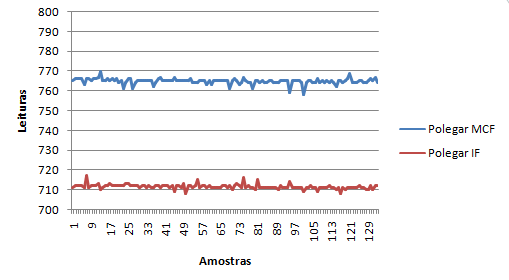
\includegraphics[width=.8\textwidth]{imagem/sensflex_pol1-2_bruto_gustavo}\label{fig:sensflexgus}}\\
  %\subfloat[Leituras obtidas com o circuito e código deste  trabalho]{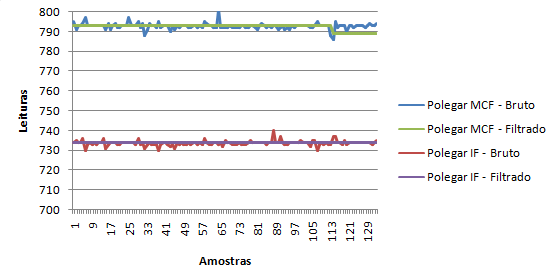
\includegraphics[width=.6\textwidth]{imagem/sensflex_pol1-2_filtrado_bruto_meu}\label{fig:sensflexmeu}}
  \captionsetup{justification=centering}
  \captionfont{\small{\textbf{\\Fonte: Elaborado pelo Autor}}}
  \label{fig:graf_sensflex}
\end{grafico}

\begin{grafico}[H]
    \ContinuedFloat
  \setlength{\abovecaptionskip}{0pt}
  \setlength{\belowcaptionskip}{0pt}
  \caption[Leituras dos sensores de flexão do polegar (Cont.)]{Leituras dos sensores de flexão do polegar (Cont.)}
  \centering
  %\subfloat[Leituras obtidas com circuito e código de \citeonline{roversi}]{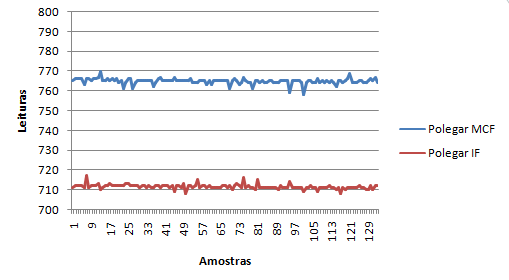
\includegraphics[width=.6\textwidth]{imagem/sensflex_pol1-2_bruto_gustavo}\label{fig:sensflexgus}}\\
  \subfloat[Leituras obtidas com o circuito e código deste  trabalho]{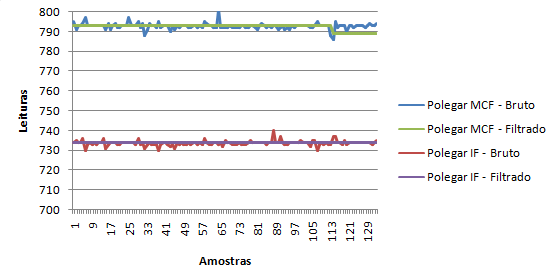
\includegraphics[width=.85\textwidth]{imagem/sensflex_pol1-2_filtrado_bruto_meu}\label{fig:sensflexmeu}}
  \captionsetup{justification=centering}
  \captionfont{\small{\textbf{\\Fonte: Elaborado pelo Autor}}}
  \label{fig:graf_sensflex2}
\end{grafico}

O \textit{MPU-6050} utilizado por \citeonline{roversi} gerava muitos ruídos pois utilizava somente as leituras do acelerômetro. Isso foi solucionado utilizando o \textit{MPU-9250} e utilizando o seu processador interno, o \ac{DMP}, para realizar a fusão dos dados do acelerômetro, giroscópio e magnetômetro embutidos, o que produziu um sinal quase completamente livre de ruídos e bastante responsivo. Os Gráficos \ref{fig:grafmpu9250} e \ref{fig:grafmpu6050} foram gerados com a \textit{MPU-9250} e \textit{MPU-6050} em uma superfície plana. Pode-se perceber que as leituras da \textit{MPU-9250} com o \ac{DMP} são quase completamente livres de ruídos, enquanto que as leituras da \textit{MPU-6050} sem o \ac{DMP} são mais instáveis. Ainda se observou o efeito de \textit{drift} durante os primeiros 15 segundos de utilização da luva, enquanto as \ac{IMU}s se calibravam, mas após esse período as leituras se estabilizaram, como mostra o Gráfico \ref{fig:grafdrift}.

\begin{grafico}[H]
  \setlength{\abovecaptionskip}{0pt}
  \setlength{\belowcaptionskip}{0pt}
  \caption[Leituras das \ac{IMU}s]{Leituras das \ac{IMU}s}
  \centering
  \subfloat[Leituras da \textit{MPU-6050} sem \ac{DMP}]{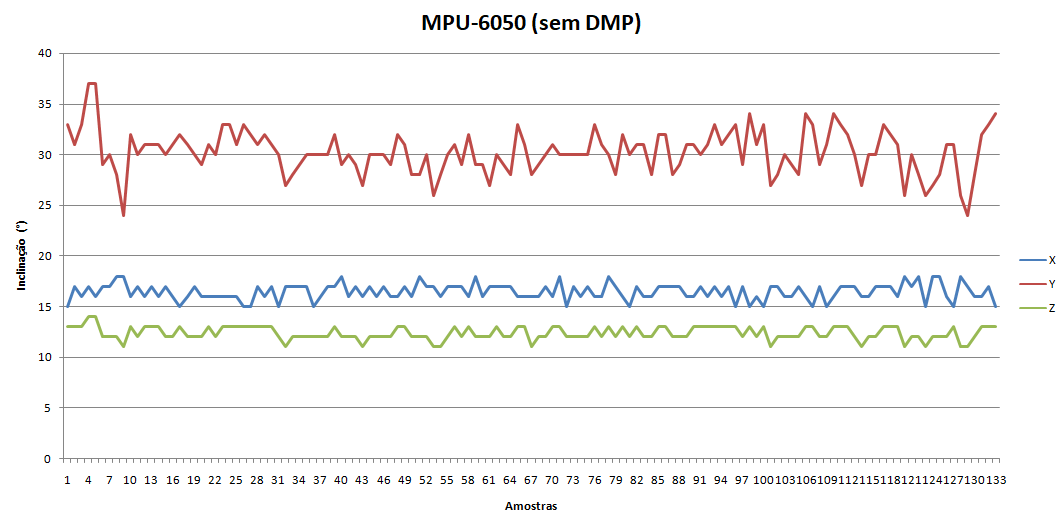
\includegraphics[trim=0 0 0 28 ,clip,width=.7\textwidth]{imagem/6050nodmp_plano.png}\label{fig:grafmpu6050}}\\
  %\subfloat[Leituras da \textit{MPU-9250} com \ac{DMP}]{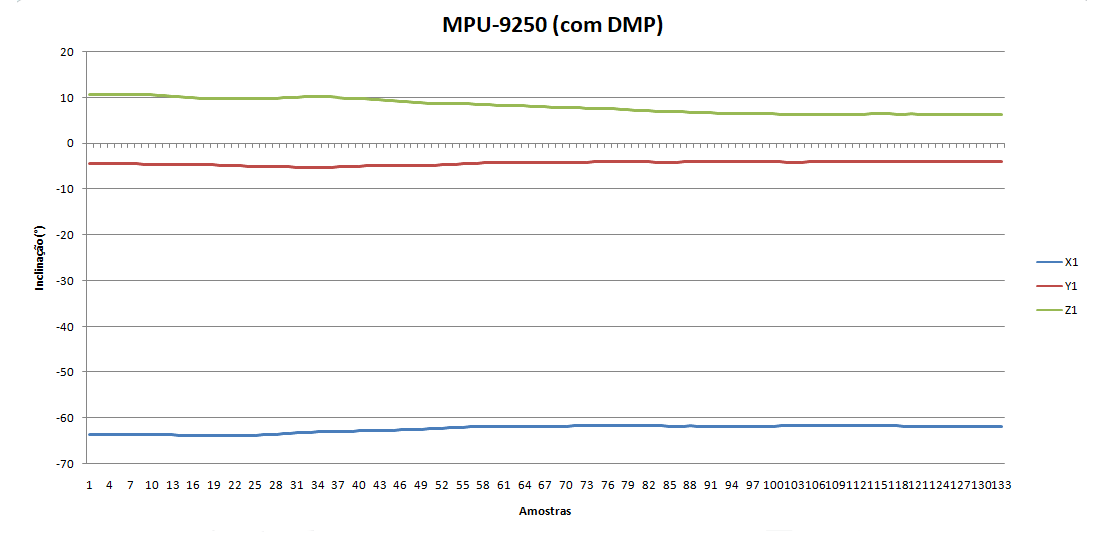
\includegraphics[trim=0 0 0 30 ,clip,width=.7\textwidth]{imagem/9250dmp_plano.png}\label{fig:grafmpu9250}}
  \captionsetup{justification=centering}
  \captionfont{\small{\textbf{\\Fonte: Elaborado pelo Autor}}}
  \label{fig:graf_mpu}
\end{grafico}

\begin{grafico}[H]
\ContinuedFloat
  \setlength{\abovecaptionskip}{0pt}
  \setlength{\belowcaptionskip}{0pt}
  \caption[Leituras das \ac{IMU}s]{Leituras das \ac{IMU}s}
  \centering
  %\subfloat[Leituras da \textit{MPU-6050} sem \ac{DMP}]{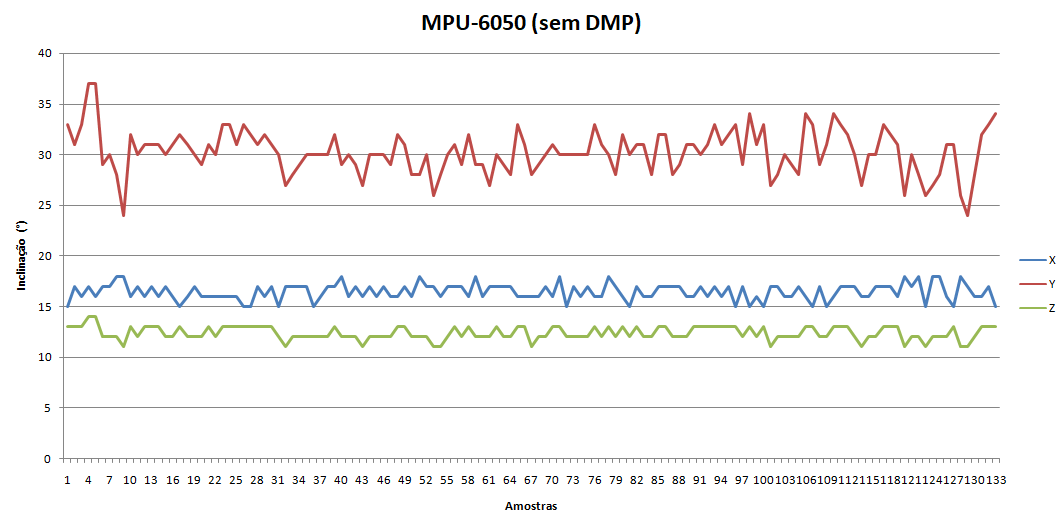
\includegraphics[trim=0 0 0 28 ,clip,width=.7\textwidth]{imagem/6050nodmp_plano.png}\label{fig:grafmpu6050}}\\
  \subfloat[Leituras da \textit{MPU-9250} com \ac{DMP}]{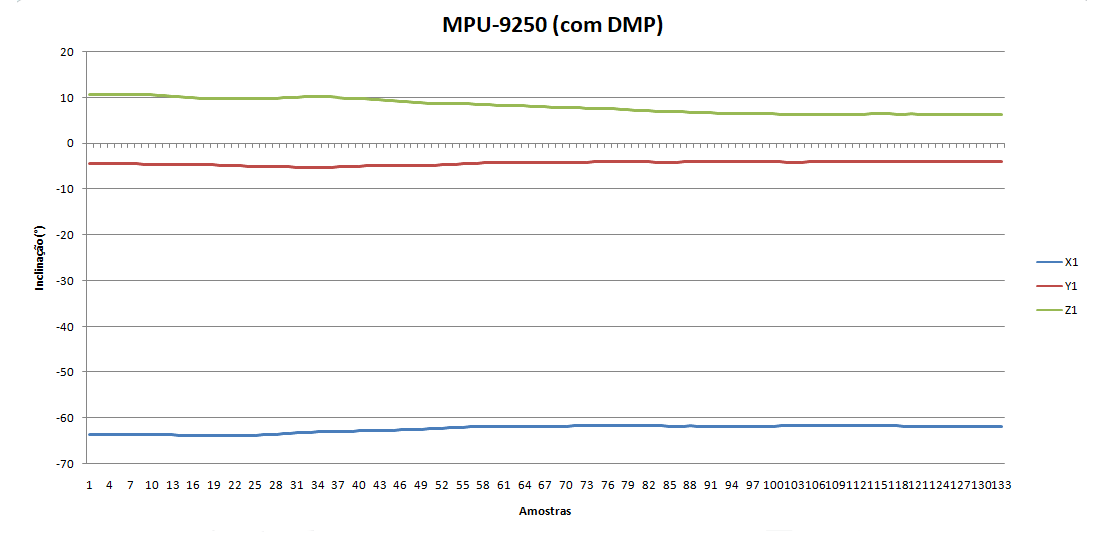
\includegraphics[trim=0 0 0 30 ,clip,width=.7\textwidth]{imagem/9250dmp_plano.png}\label{fig:grafmpu9250}}
  \captionsetup{justification=centering}
  \captionfont{\small{\textbf{\\Fonte: Elaborado pelo Autor}}}
  \label{fig:graf_mpu2}
\end{grafico}

\begin{grafico}[H]
  \setlength{\abovecaptionskip}{0pt}
  \setlength{\belowcaptionskip}{0pt}
  \caption[Efeito \textit{drift} da \textit{MPU-9250}]{Efeito \textit{drift} da \textit{MPU-9250}}
  \centering
  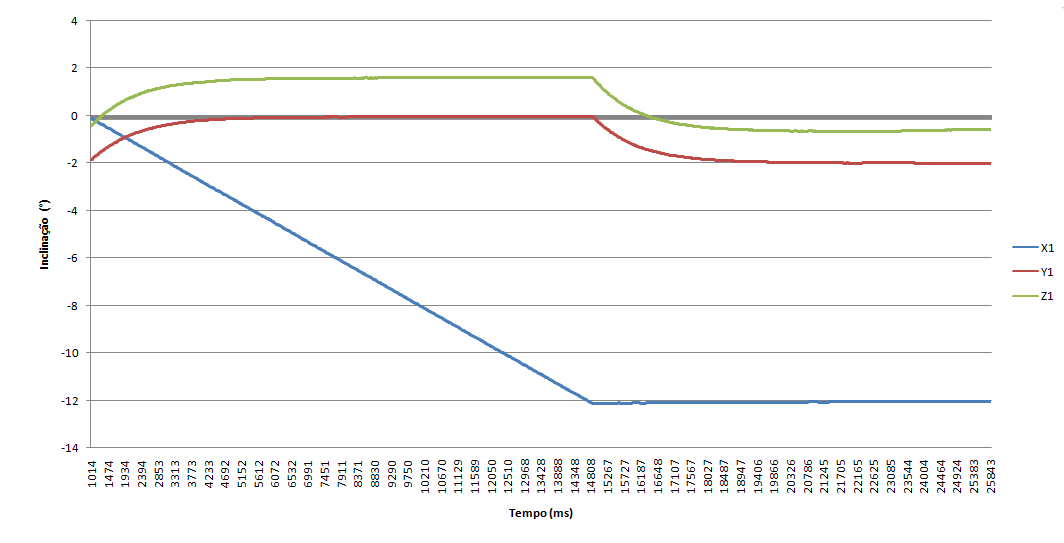
\includegraphics[width=.7\textwidth]{imagem/drift_mpu1.png}
  \captionsetup{justification=centering}
  \captionfont{\small{\textbf{\\Fonte: Elaborado pelo Autor}}}
  \label{fig:grafdrift}
\end{grafico}

A Tabela \ref{tab:imu_est_plan} mostra a análise dos ângulos obtidos pelas \ac{IMU}s com a mão e o braço na posição plana. Os cálculos para as \ac{IMU}s deste trabalho foram feitos utilizando a diferença entre os ângulos obtidos das \textit{MPU-9250} do braço e da mão e, os cálculos para a \ac{IMU} de \citeonline{roversi} foram feitos com as devidas conversões dos dados da \textit{MPU-6050}. Nota-se uma redução do \ac{DP}, o que sugere que o \ac{DMP} da \textit{MPU-9250} foi suficiente para redução de ruídos e suavização dos movimentos. Percebe-se também que o \ac{DMA} atingiu uma diferença de até \ang{15}, o que foi causado devido ao mau posicionamento do \textit{Arduino} no braço, pois o mesmo tendia a ficar inclinado em relação à \ac{IMU} da mão.

\begin{table}[H]
  \centering
  \footnotesize
  \setlength{\abovecaptionskip}{0pt}
  \setlength{\belowcaptionskip}{0pt}
  \caption[Análise das leituras das \ac{IMU}s na posição plana]{Análise das leituras das \ac{IMU}s na posição plana}
  \label{tab:imu_est_plan}
\begin{tabular}{l|rrrr|rrrr}
    \hline\hline
	\multirow{2}{*}{Sensor} & \multicolumn{4}{c|}{Este Trabalho - \textit{MPU-9250}} & \multicolumn{4}{c}{\citeonline{roversi} - \textit{MPU-6050}} \\
	\cline{2-9}
    \multirow{1}{*}{} & \multicolumn{1}{c}{Média} & \multicolumn{1}{c}{\ac{DP}} & \multicolumn{1}{c}{Amplitude} & \multicolumn{1}{c|}{\ac{DMA}} & 
    \multicolumn{1}{c}{Média} & 
    \multicolumn{1}{c}{\ac{DP}} & \multicolumn{1}{c}{Amplitude} & \multicolumn{1}{c}{\ac{DMA}} \\
    \hline
IMU - eixo X & -15,276 & 0,680 & 2,280 & 15,165 & 9,263 & 1,630 & 1,500 & 9,263 \\
IMU - eixo Y & -8,108 & 0,466 & 2,110 & 8,005 & 2,398 & 3,051 & 5,000 & 2,398 \\
IMU - eixo Z & 18,167 & 0,707 & 2,160 & 8,332 & 21,327 & 1,220 & 1,500 & 21,327 \\
    \hline\hline
\end{tabular}
  \\\vspace{1.3mm}
  \captionfont{\small{\textbf{Fonte: Elaborado pelo Autor}}}
\end{table}

A Tabela \ref{tab:an_est_ger} mostra as médias do \ac{DP}, Amplitude e \ac{DMA} dos sensores para cada repetição de cada movimento. As posições 1, 2, 3, 4 e 9 foram calculadas com os dados dos sensores de flexão e as posições 5, 6, 7 e 8 forma calculadas com os dados das \ac{IMU}s. Percebe-se que as leituras possuíram \ac{DP} e amplitude menores, indicando que o filtro aplicado reduziu as oscilações indesejadas do modelo. Além disso, a luva deste trabalho possui um \ac{DMA} menor, indicando que os movimentos realizados foram mais precisos que as de \citeonline{roversi}, pois os ângulos calculados forma mais próximos dos ângulos reais.
\begin{table}[H]
  \centering
  \footnotesize
  \setlength{\abovecaptionskip}{0pt}
  \setlength{\belowcaptionskip}{0pt}
  \caption[Análise geral das leituras dos sensores para cada movimento]{Análise geral das leituras dos sensores para cada movimento}
  \label{tab:an_est_ger}
\begin{tabular}{l|rrr|rrr}
\hline\hline
\multirow{2}{*}{Posições} & \multicolumn{3}{c|}{Este Trabalho} & \multicolumn{3}{c}{\citeonline{roversi}} \\
\cline{2-7}
\multirow{1}{*}{} & \multicolumn{1}{c}{\ac{DP}} & \multicolumn{1}{c}{Amplitude} & \multicolumn{1}{c|}{\ac{DMA}} & \multicolumn{1}{c}{\ac{DP}} & \multicolumn{1}{c}{Amplitude} & \multicolumn{1}{c}{\ac{DMA}} \\
\hline			
1 (Mão plana)                  & 0,442  & 2,286  & 5,829  & 0,812  & 7,500  & 2,160 \\
2 (Flexão MCF e IF do polegar) & 0,069  & 0,333  & 7,000  & 2,534  & 15,500 & 10,337 \\
3 (Flexão MCF dos dedos)       & 0,848  & 4,167  & 9,038  & 3,366  & 18,667 & 17,403 \\
4 (Flexão IFP dos dedos)       & 0,301  & 0,667  & 9,209  & 3,551  & 16,000 & 18,840 \\
5 (Extensão do pulso)          & 0,428  & 2,560  & 5,014  & 0,890  & 4,833  & 27,509 \\
6 (Flexão do pulso)            & 0,635  & 2,980  & 4,608  & 0,892  & 4,500  & 5,046 \\
7 (Desvio Ulnar)               & 0,360  & 1,333  & 7,374  & --     & --     & -- \\
8 (Desvio Radial)              & 0,111  & 0,547  & 7,836  & --     & --     & -- \\
9 (Abdução dos dedos)          & 0,239  & 1,180  & 1,800  & --     & --     & -- \\
\hline
Média                          & 0,382  & 1,784  & 6,412  & 2,008  & 11,167 & 13,549 \\
\hline\hline
\end{tabular}
  \\\vspace{1.3mm}
  \captionfont{\small{\textbf{Fonte: Elaborado pelo Autor}}}
\end{table}


O método de comunicação do \textit{Arduino} com a \textit{Unity} no trabalho de \citeonline{roversi} fazia com que muitos dados ficassem presos no \textit{buffer} de entrada da porta serial do computador devido à velocidade de envio. A solução desse trabalho foi que a \textit{Unity} requisitasse os dados ao \textit{Arduino} a cada atualização de \textit{frame}.  Apesar de haver um pequeno atraso em relação ao movimento real e o movimento do modelo, essa solução se mostrou satisfatória, gerando movimentos mais fluidos, já que o modelo \ac{3D} sempre era atualizado com os dados mais recentes.

A Figura \ref{fig:pos_res} a seguir mostra a comparação dos movimentos reais e dos reproduzidos pelo modelo \ac{3D}. É possível notar nas Figuras \ref{fig:pos_3_modelo} e \ref{fig:pos_7_modelo} que a articulação \ac{IFP} do dedo indicador está ligeiramente flexionada devido a ruídos provenientes do sensor de flexão. 

\begin{figure}[H]
  \setlength{\abovecaptionskip}{0pt}
  \setlength{\belowcaptionskip}{0pt}
  \caption[Posições reais seus resultados reproduzidos pelo modelo \ac{3D}]{Posições reais seus resultados reproduzidos pelo modelo \ac{3D}}
  \centering
  \subfloat[Posição 1 - Real]{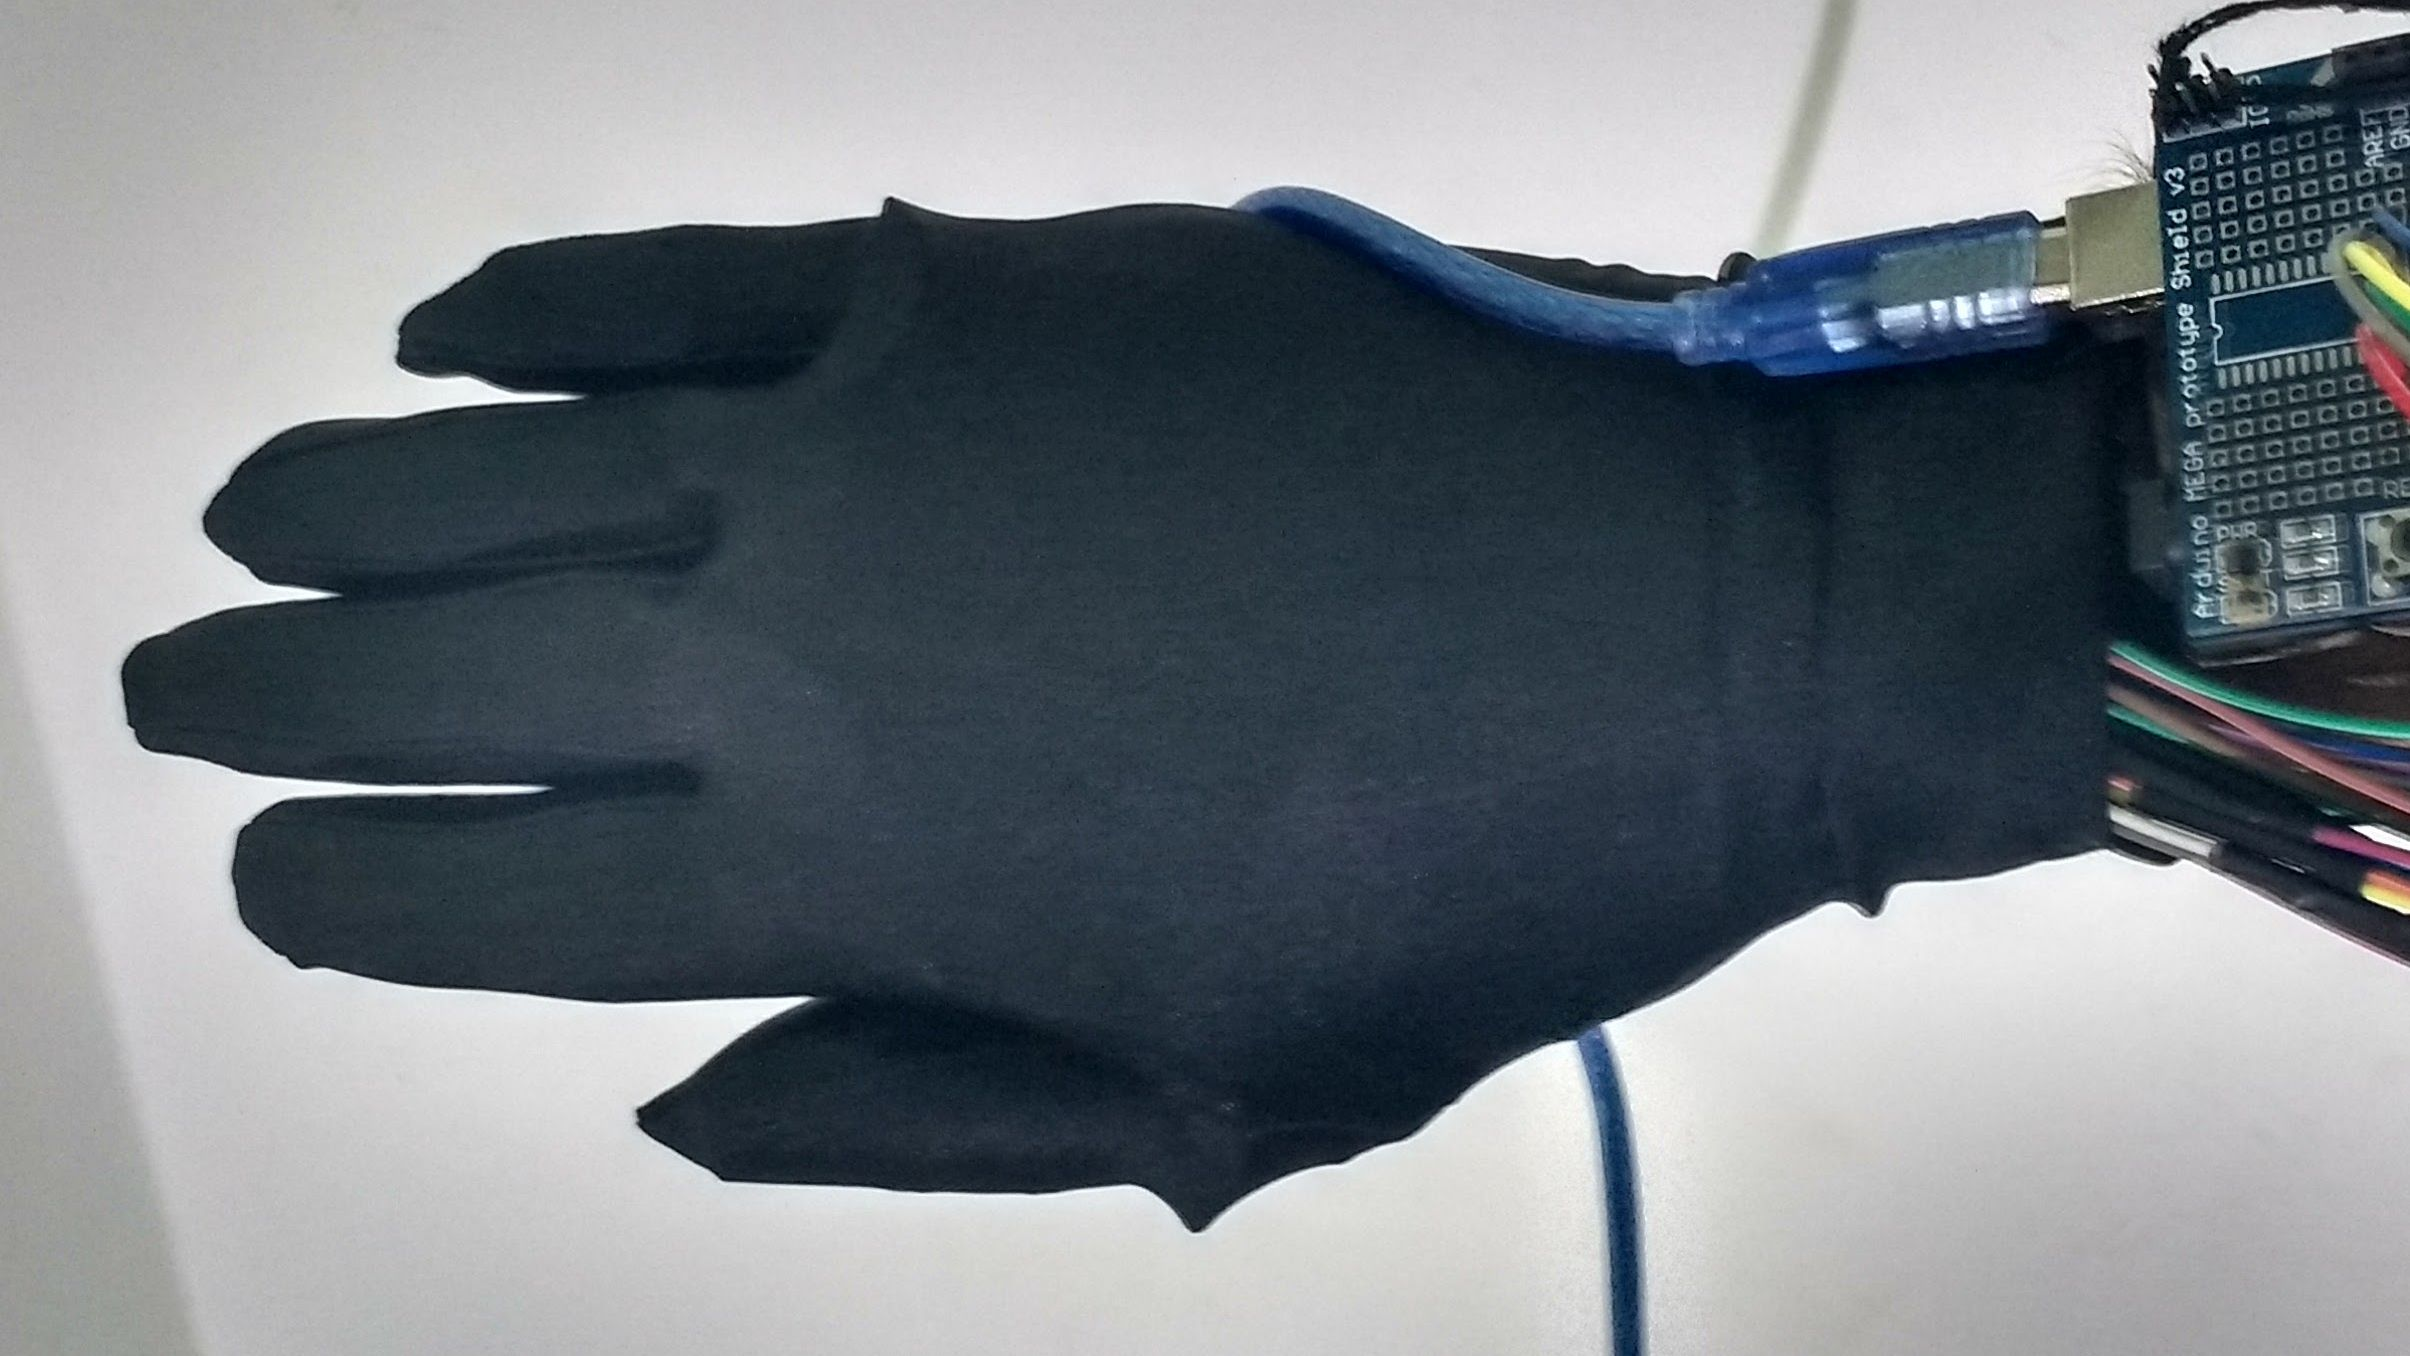
\includegraphics[width=.4\textwidth]{imagem/p1_real}\label{fig:pos_1_real}}
  \quad
  \subfloat[Posição 1 - Modelo]{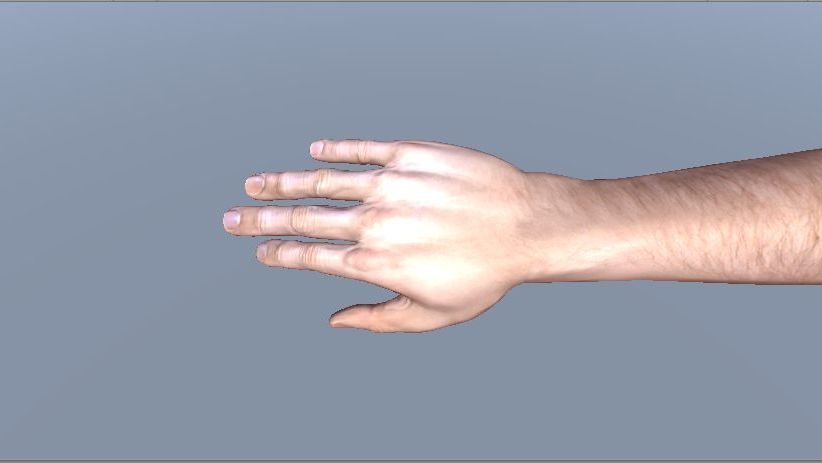
\includegraphics[width=.4\textwidth]{imagem/p1}\label{fig:pos_1_modelo}}\\
  \subfloat[Posição 2 - Real]{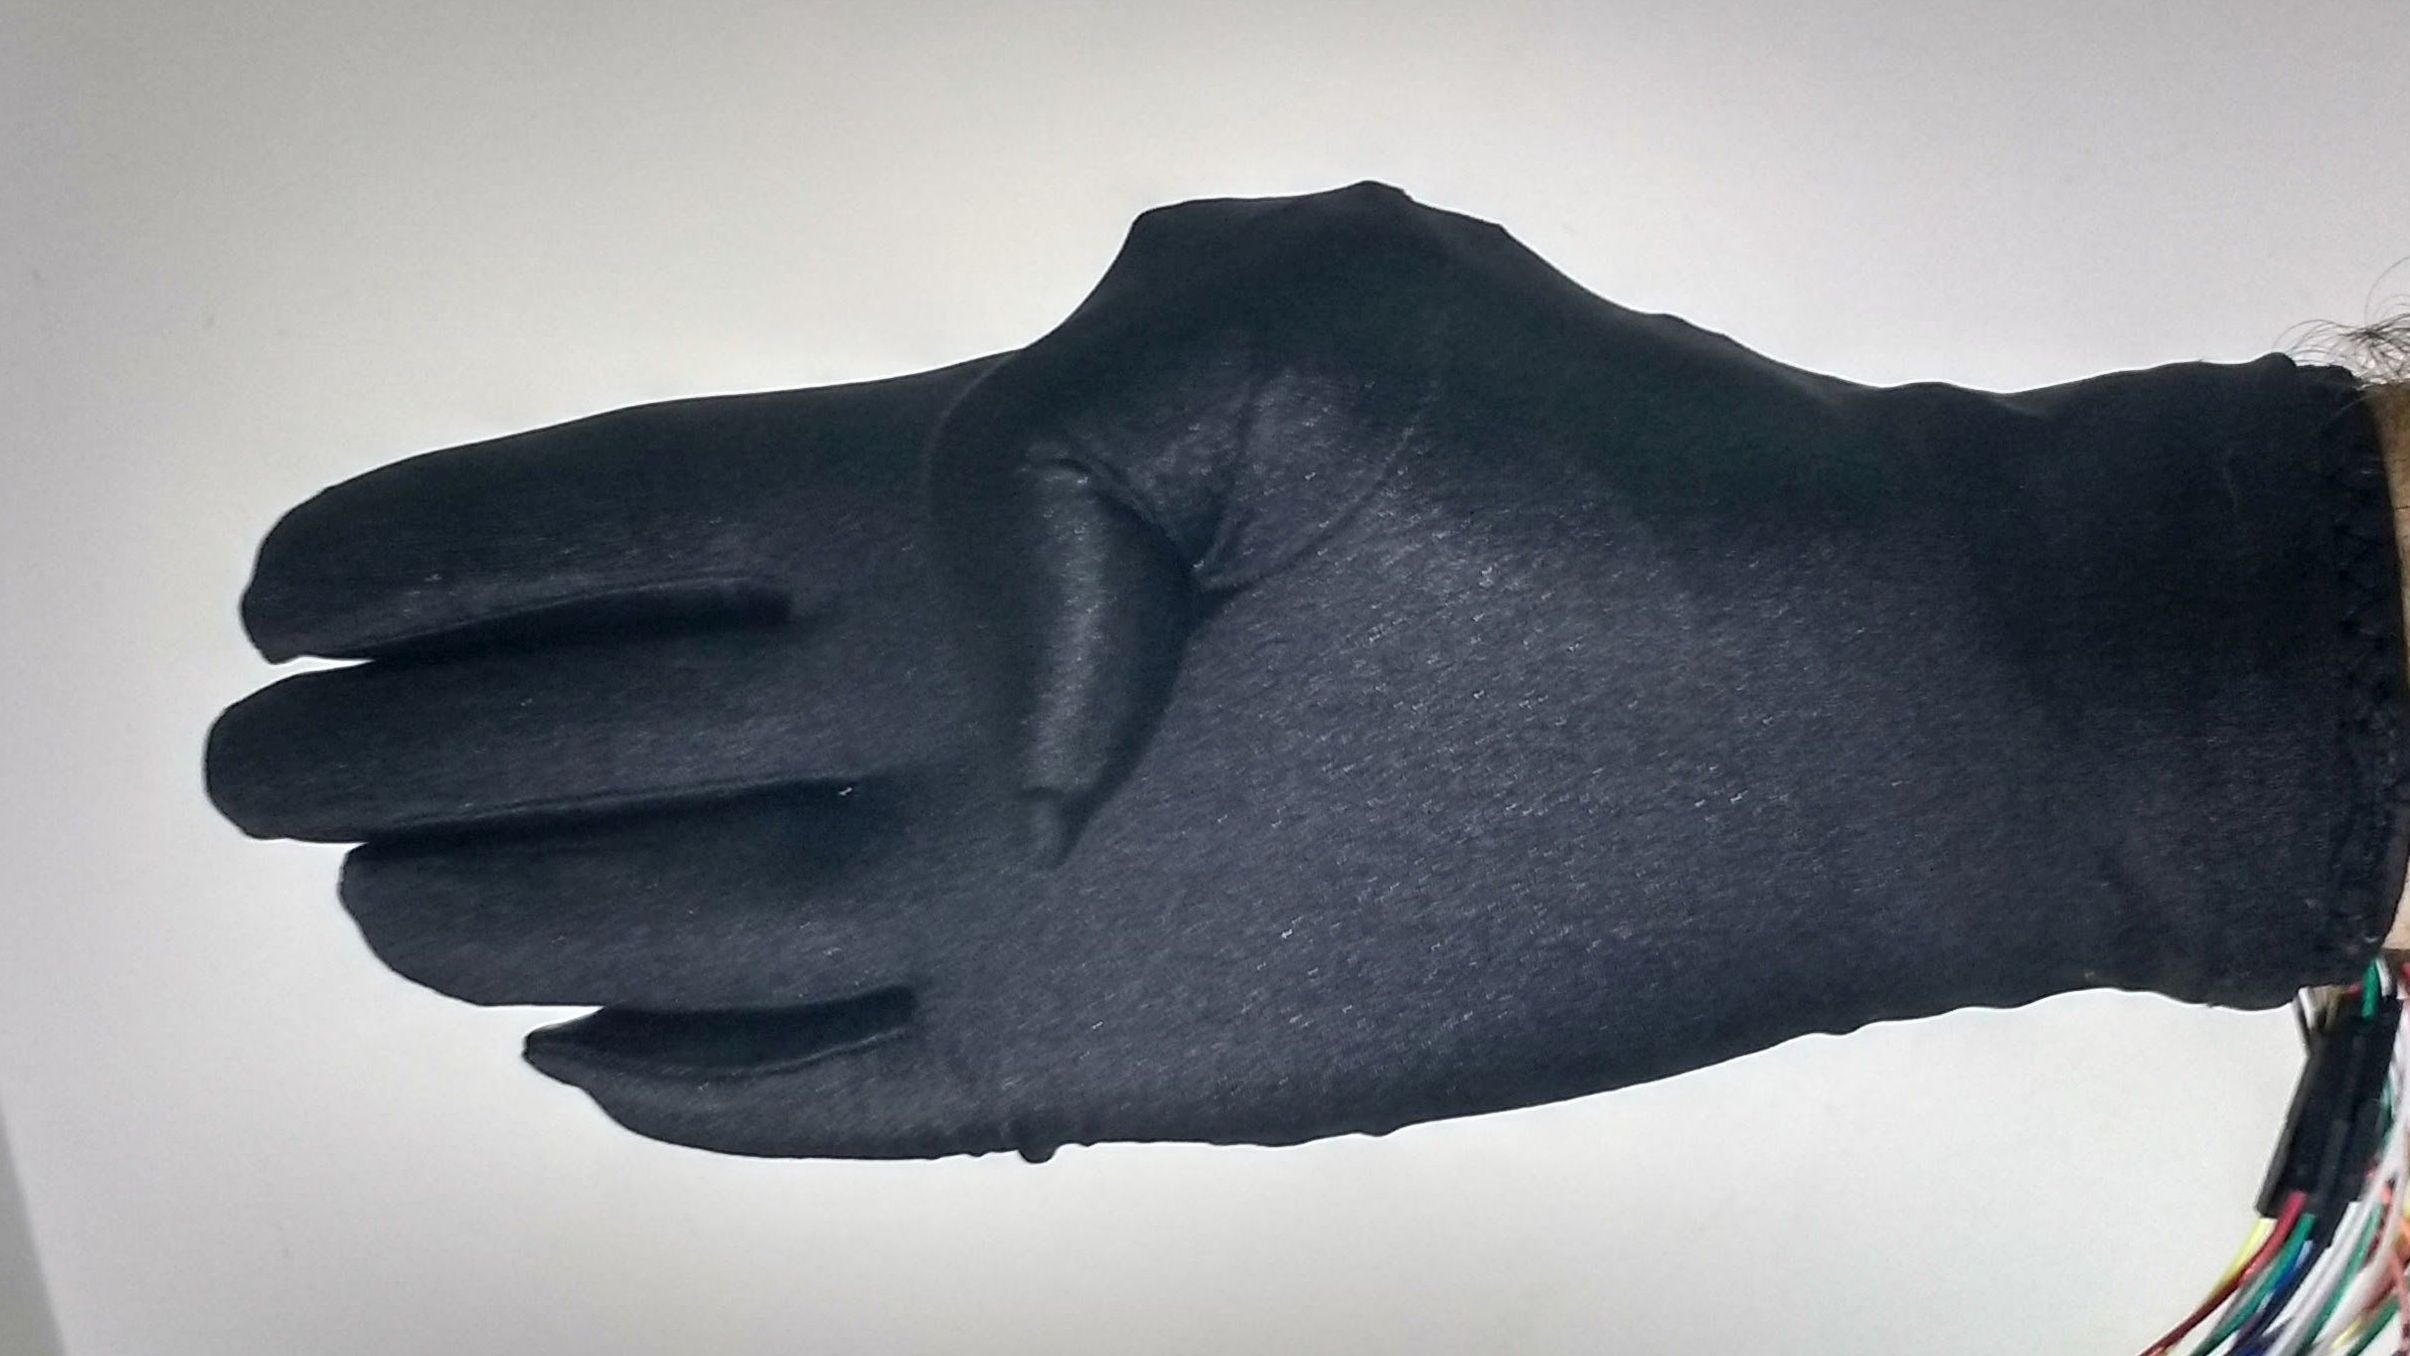
\includegraphics[width=.4\textwidth]{imagem/p2_real}\label{fig:pos_2_real}}
  \quad
  \subfloat[Posição 2 - Modelo]{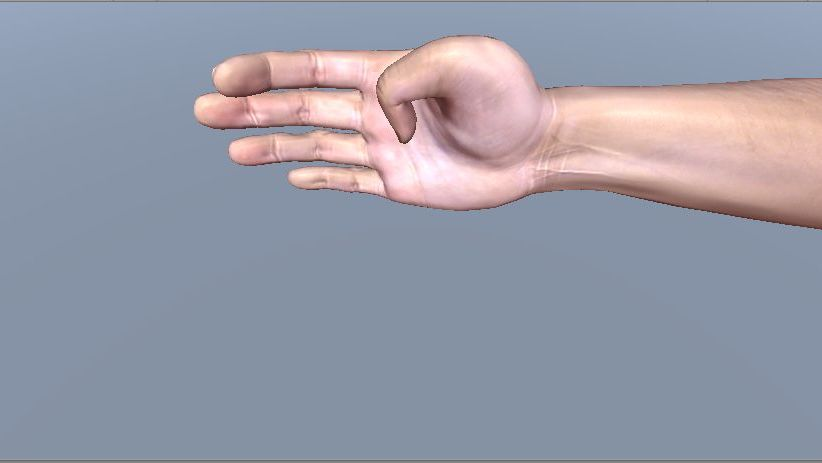
\includegraphics[width=.4\textwidth]{imagem/p2}\label{fig:pos_2_modelo}}\\
  \subfloat[Posição 3 - Real]{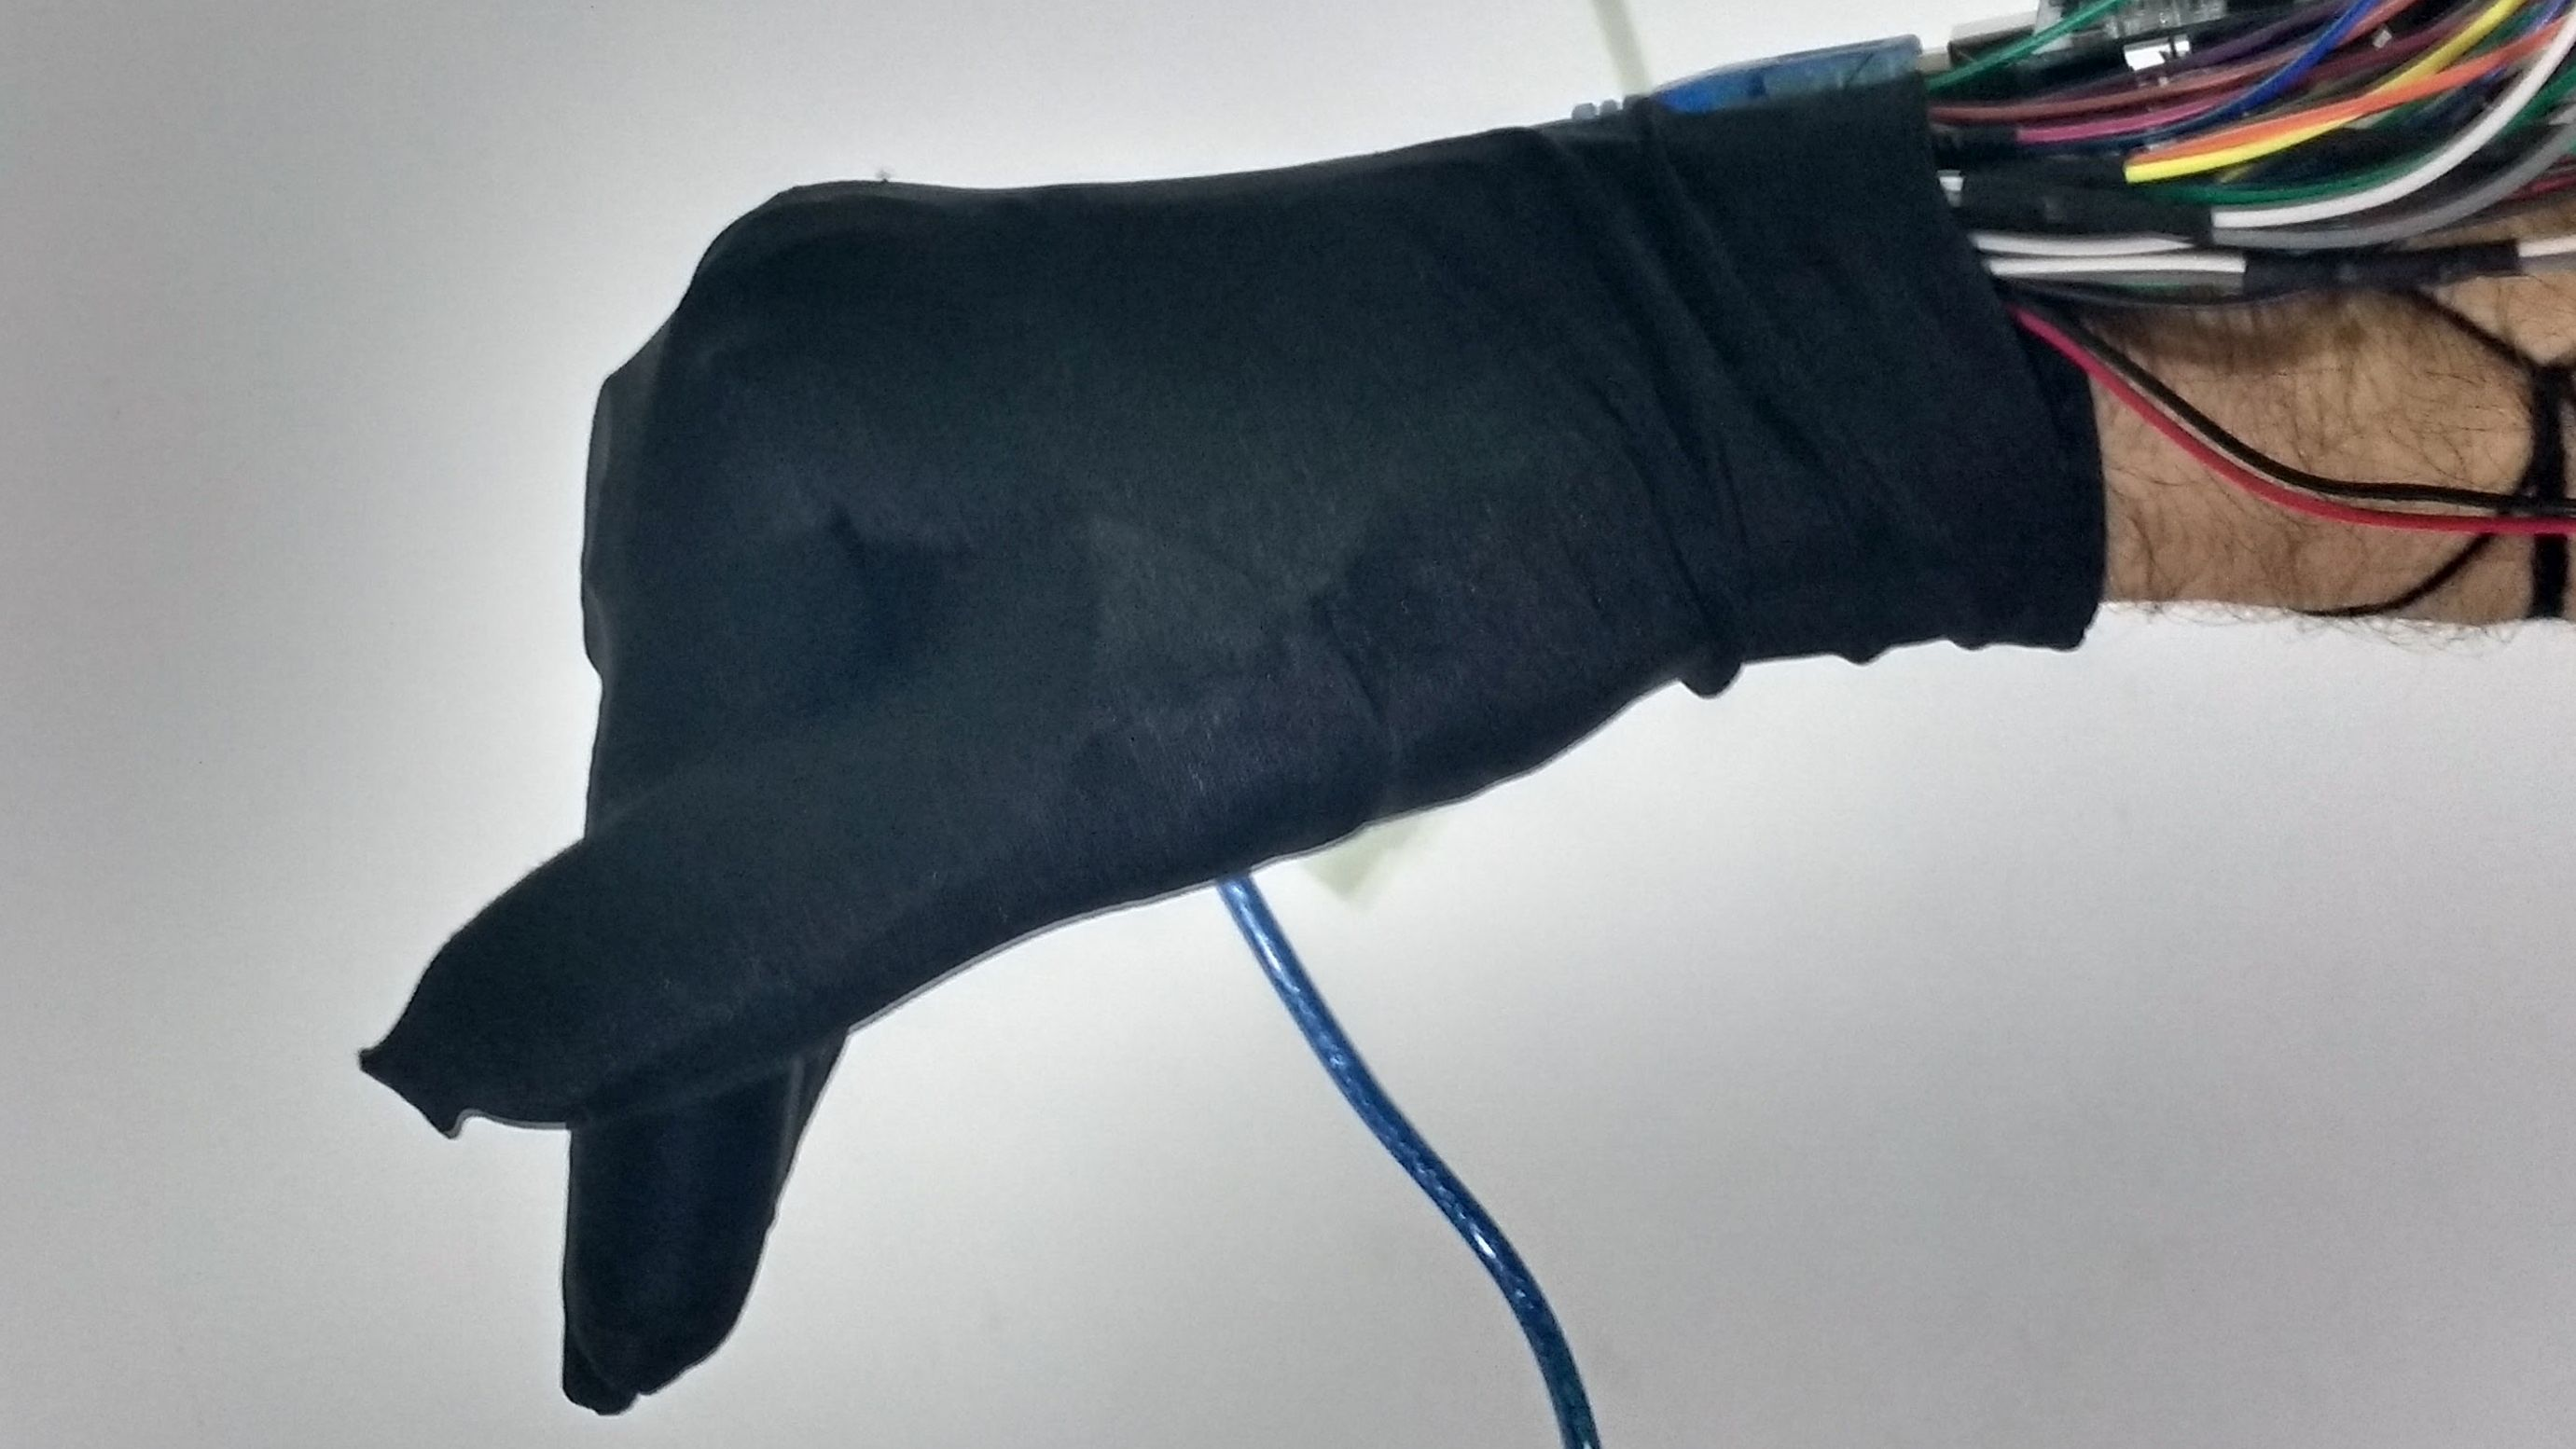
\includegraphics[width=.4\textwidth]{imagem/p3_real}\label{fig:pos_3_real}}
  \quad
  \subfloat[Posição 3 - Modelo]{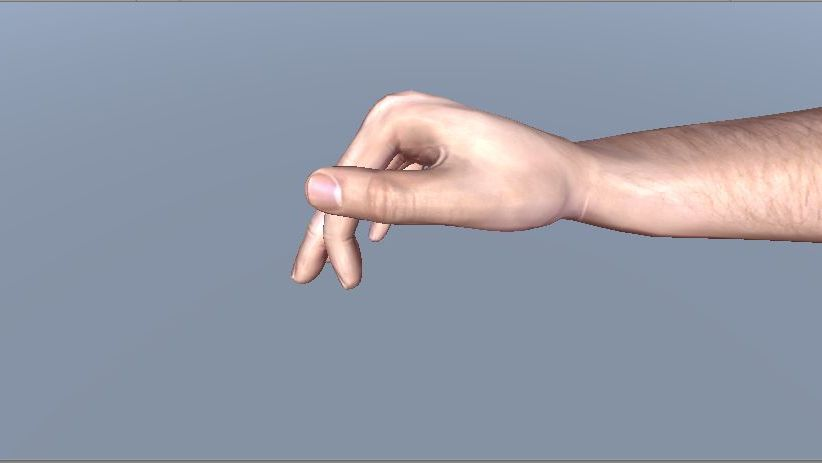
\includegraphics[width=.4\textwidth]{imagem/p3}\label{fig:pos_3_modelo}}\\
  \subfloat[Posição 4 - Real]{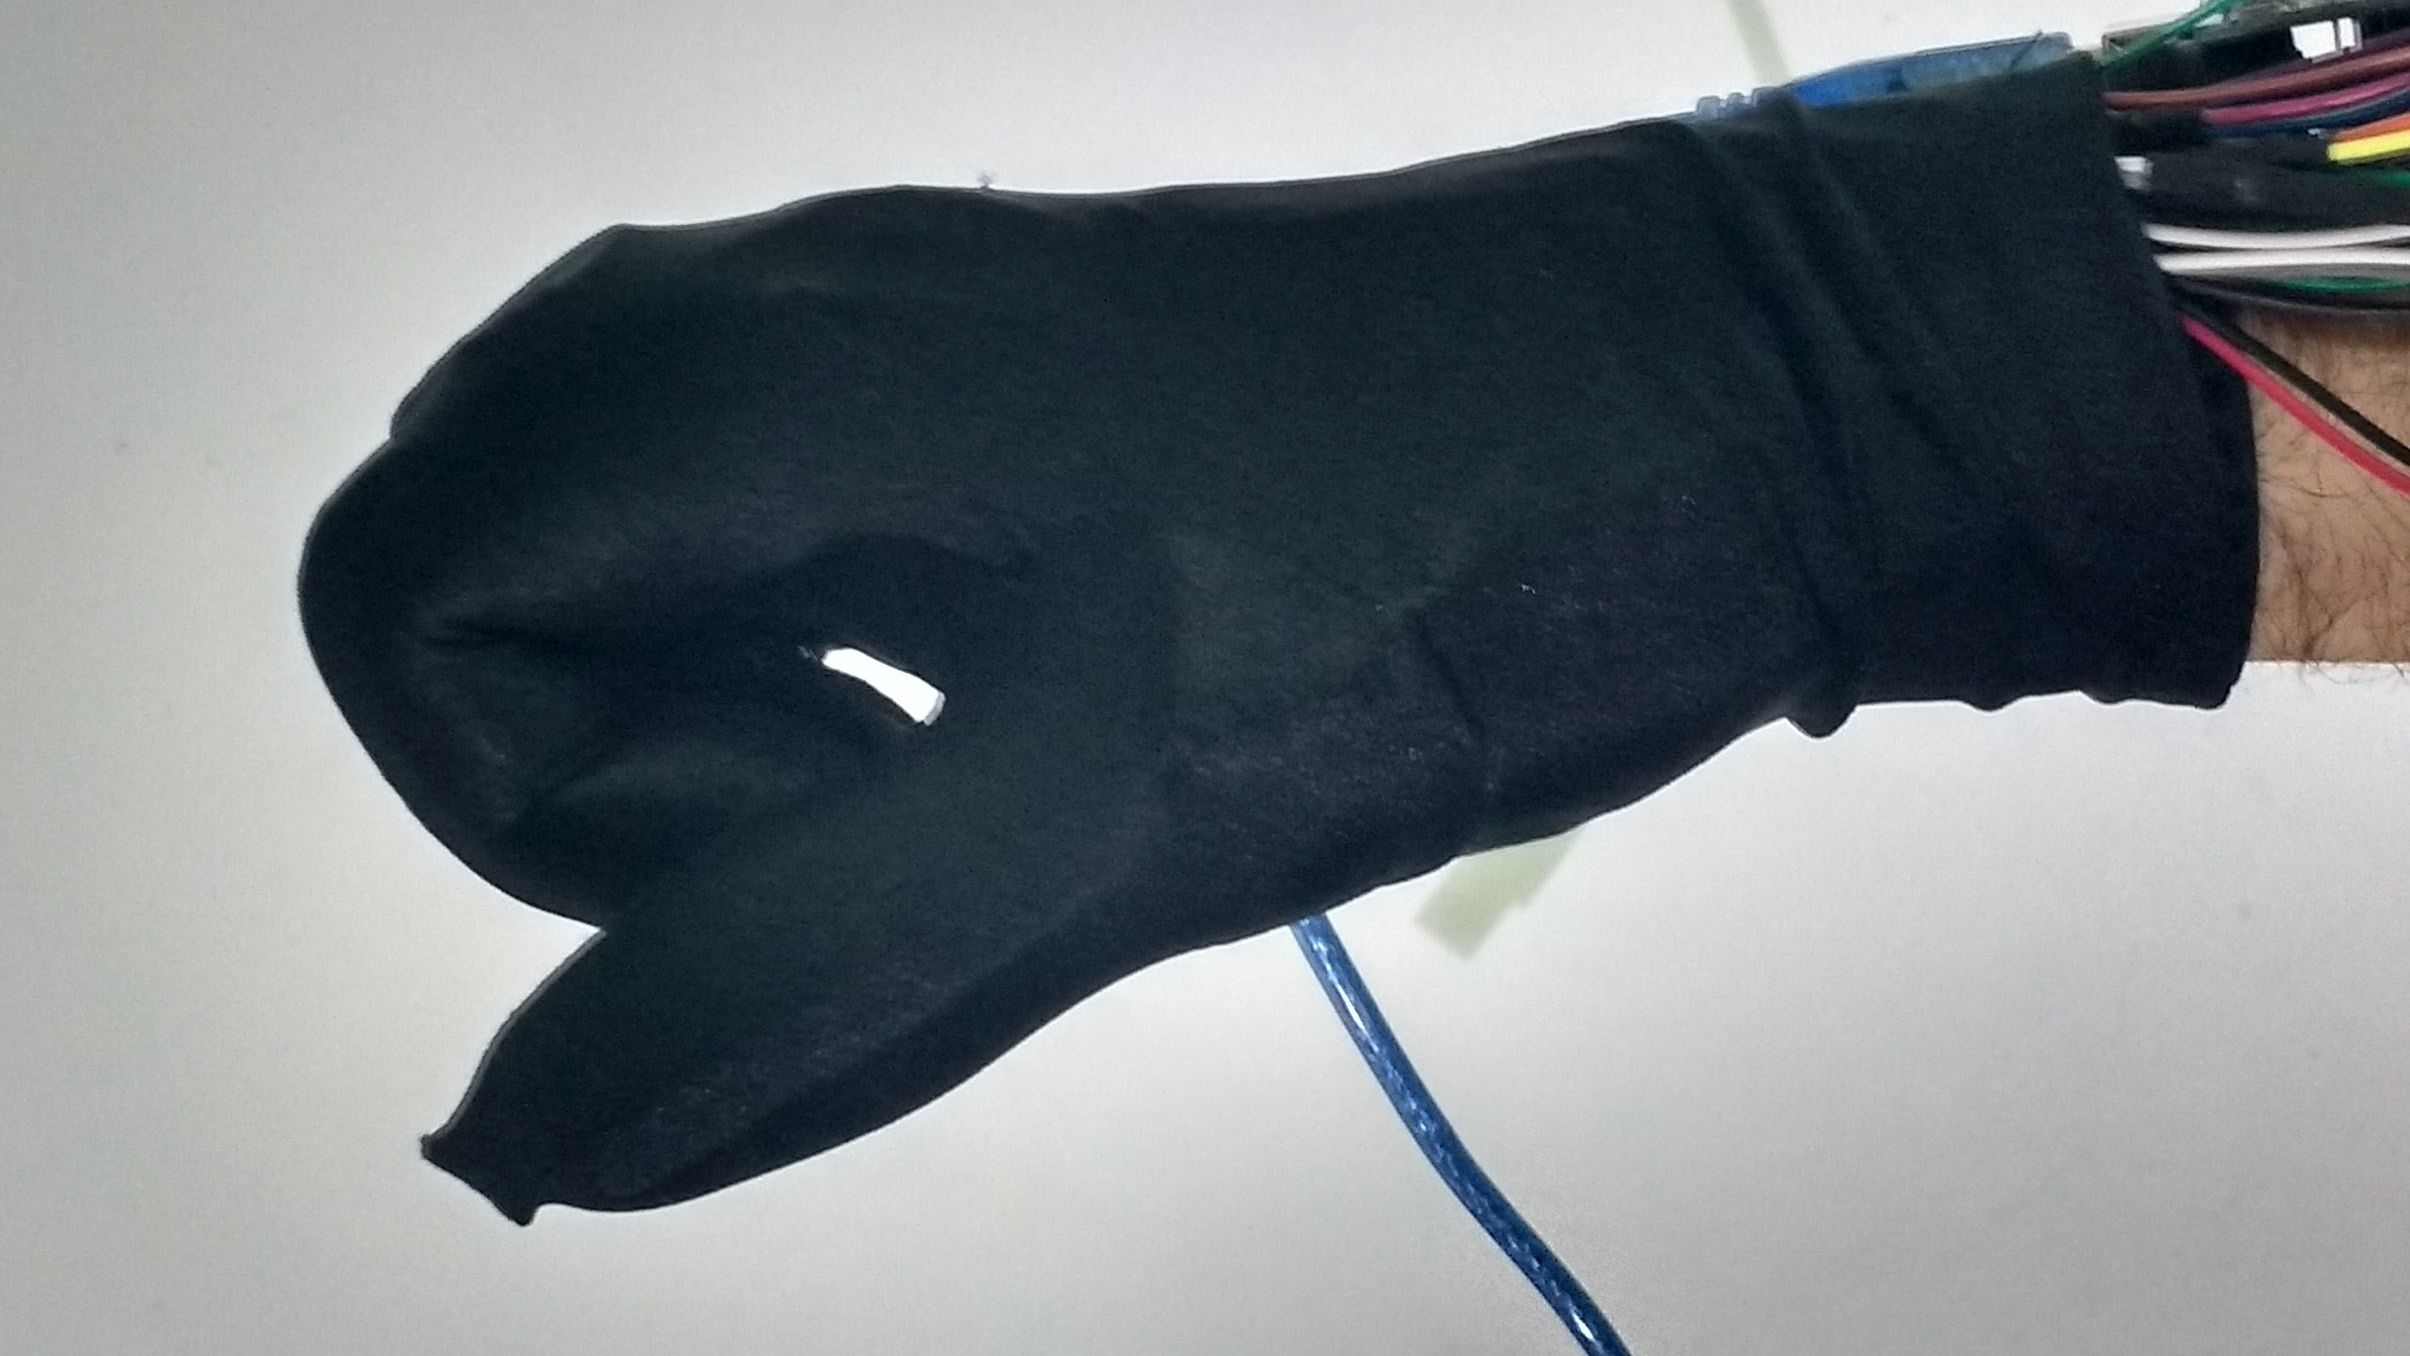
\includegraphics[width=.4\textwidth]{imagem/p4_real}\label{fig:pos_4_real}}
  \quad
  \subfloat[Posição 4 - Modelo]{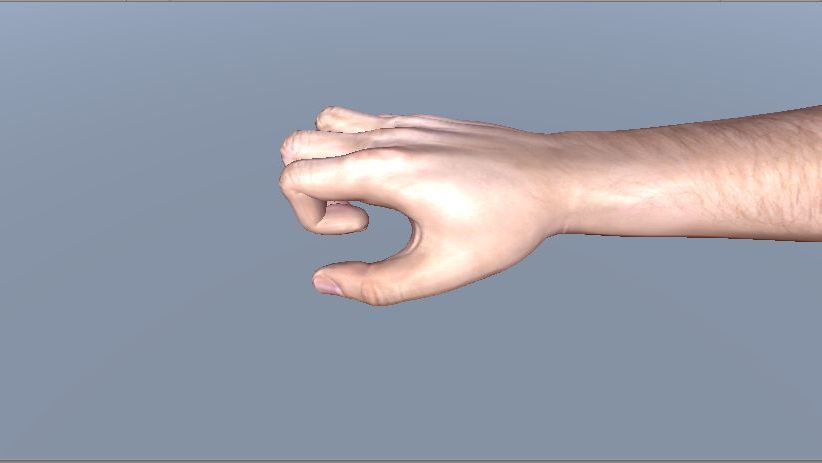
\includegraphics[width=.4\textwidth]{imagem/p4}\label{fig:pos_4_modelo}}\\
  \captionsetup{justification=centering}
  \captionfont{\small{\textbf{\\Fonte: Elaborado pelo Autor}}}
  \label{fig:pos_res}
\end{figure}

\begin{figure}[H]
  \ContinuedFloat
  \setlength{\abovecaptionskip}{0pt}
  \setlength{\belowcaptionskip}{0pt}
  \caption[Posições reais seus resultados reproduzidos pelo modelo \ac{3D}]{Posições reais seus resultados reproduzidos pelo modelo \ac{3D}}
  \centering
  \subfloat[Posição 5 - Real]{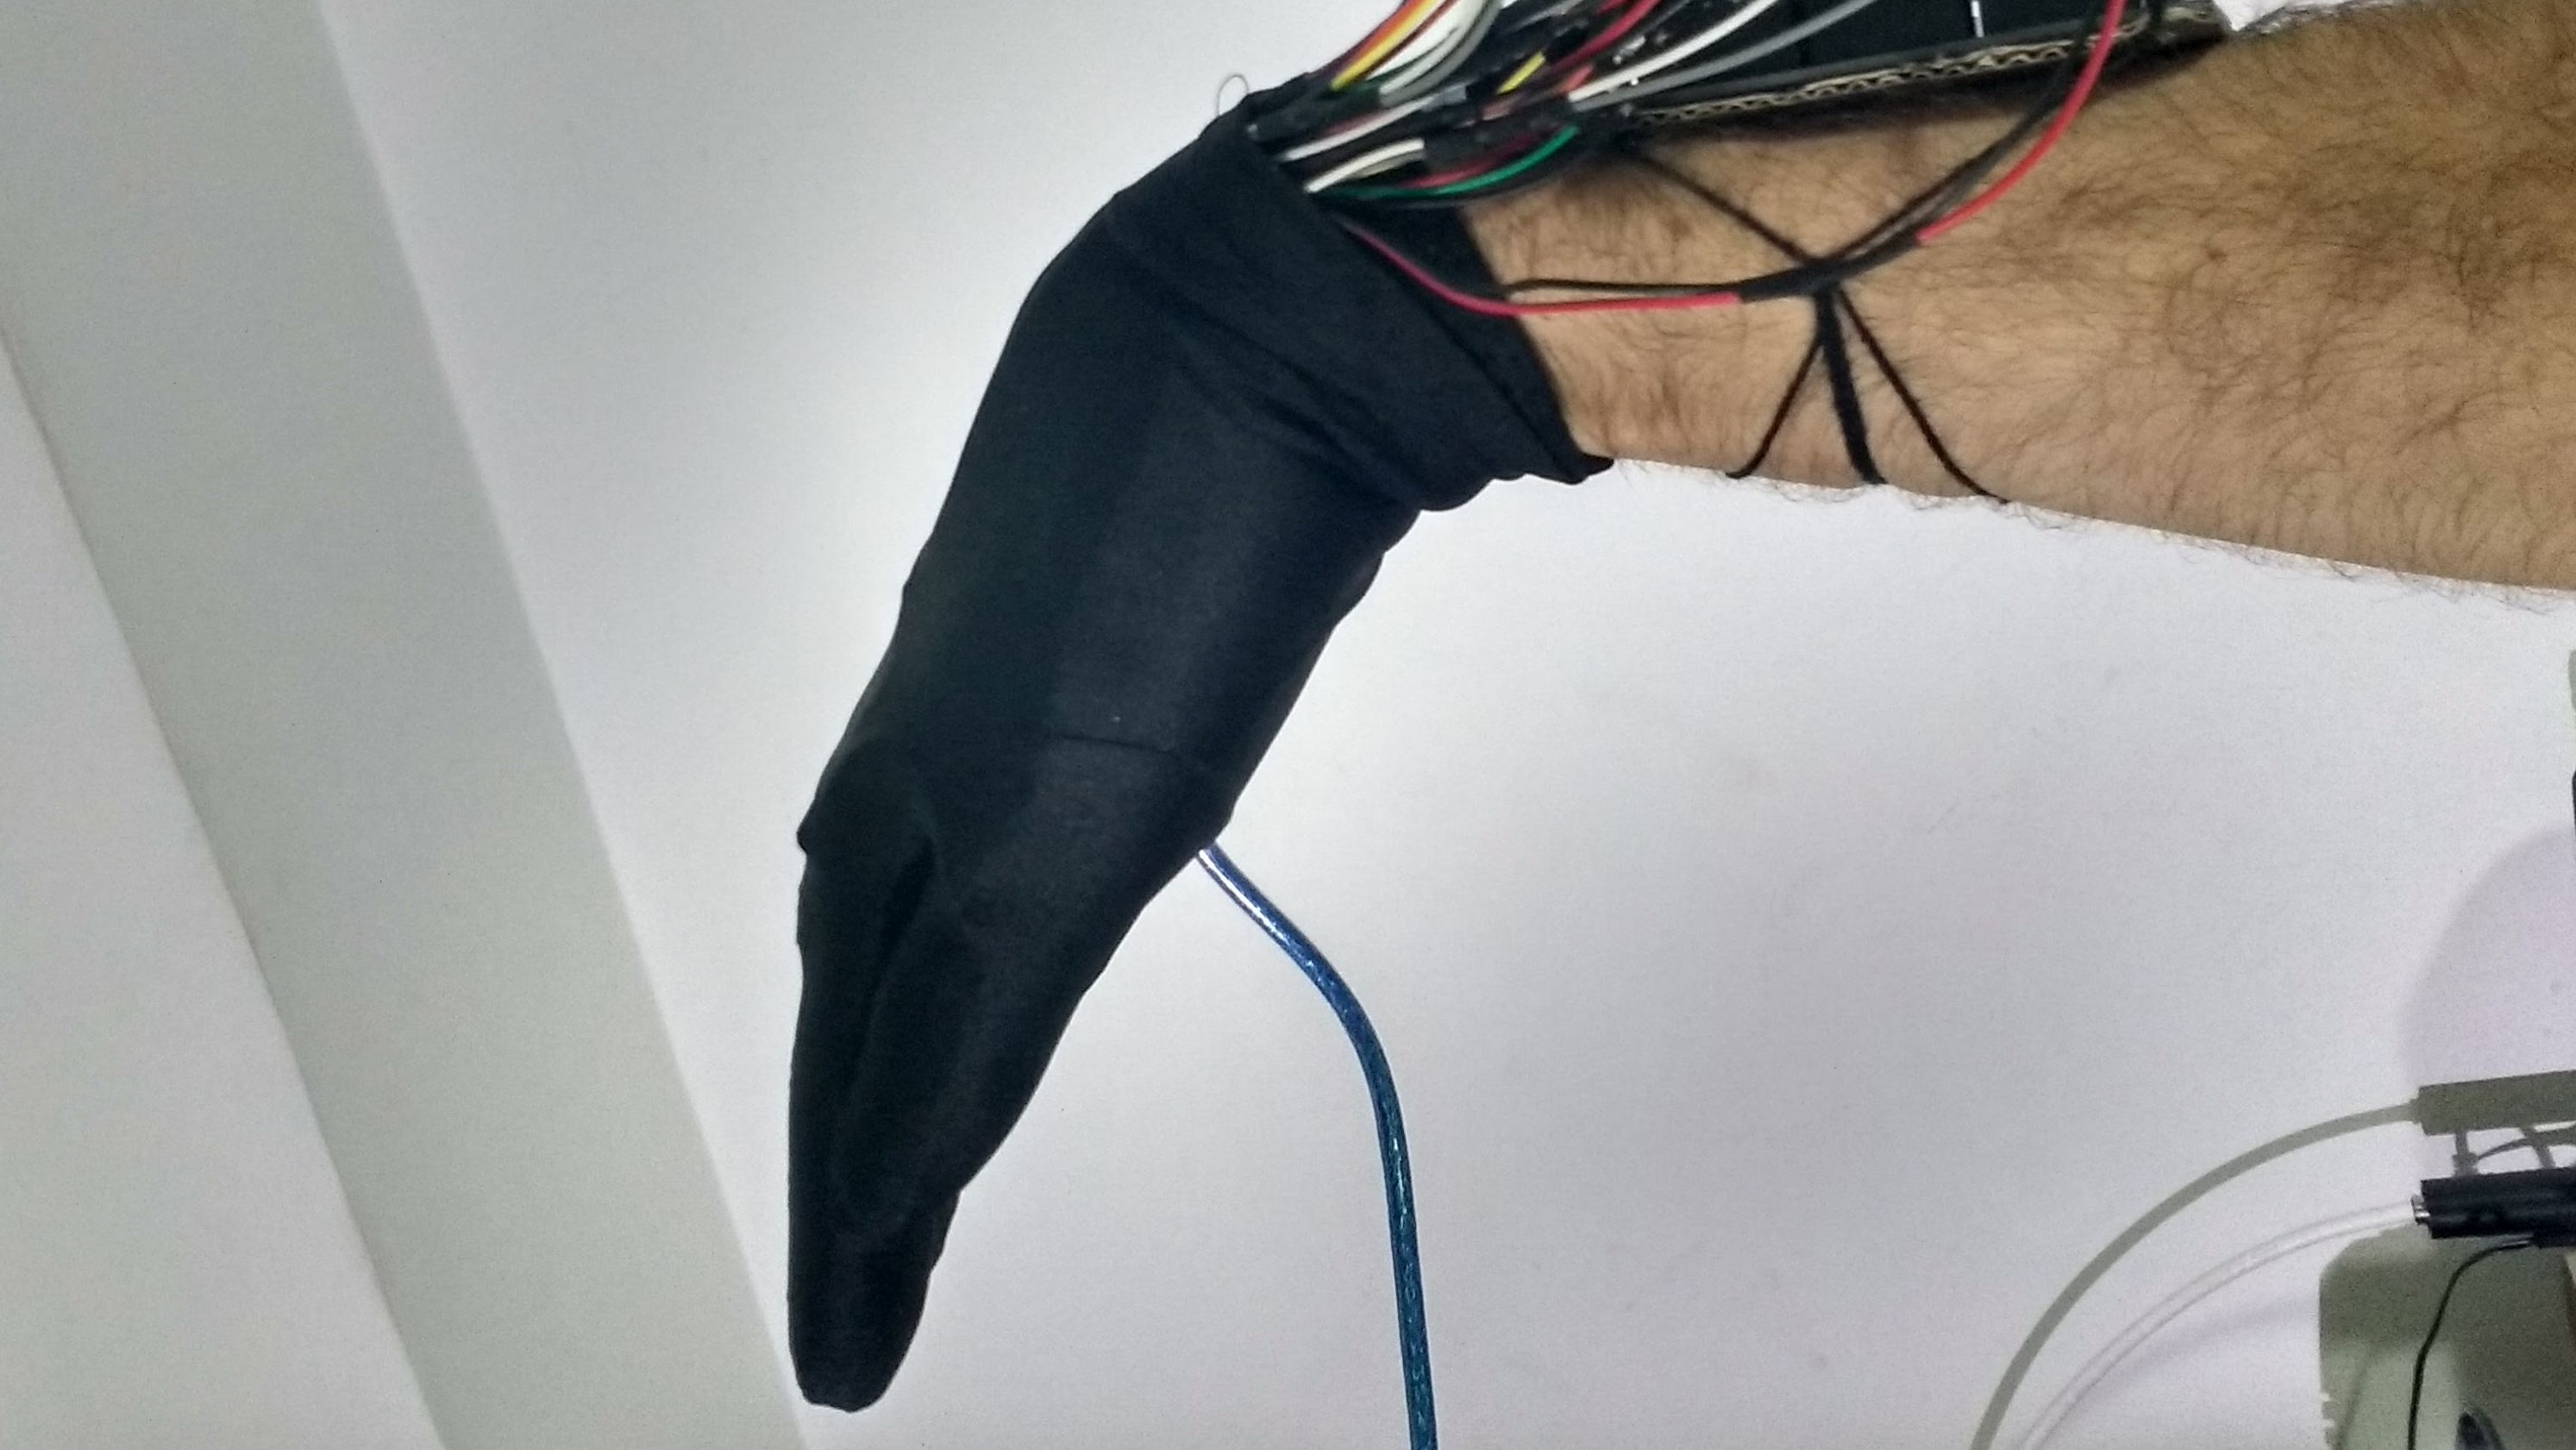
\includegraphics[width=.4\textwidth]{imagem/p5_real}\label{fig:pos_5_real}}
  \quad
  \subfloat[Posição 5 - Modelo]{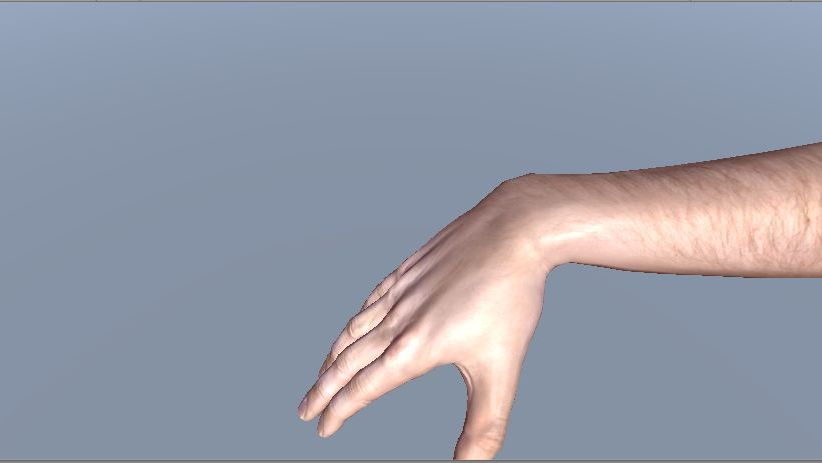
\includegraphics[width=.4\textwidth]{imagem/p5}\label{fig:pos_5_modelo}}\\
  \subfloat[Posição 6 - Real]{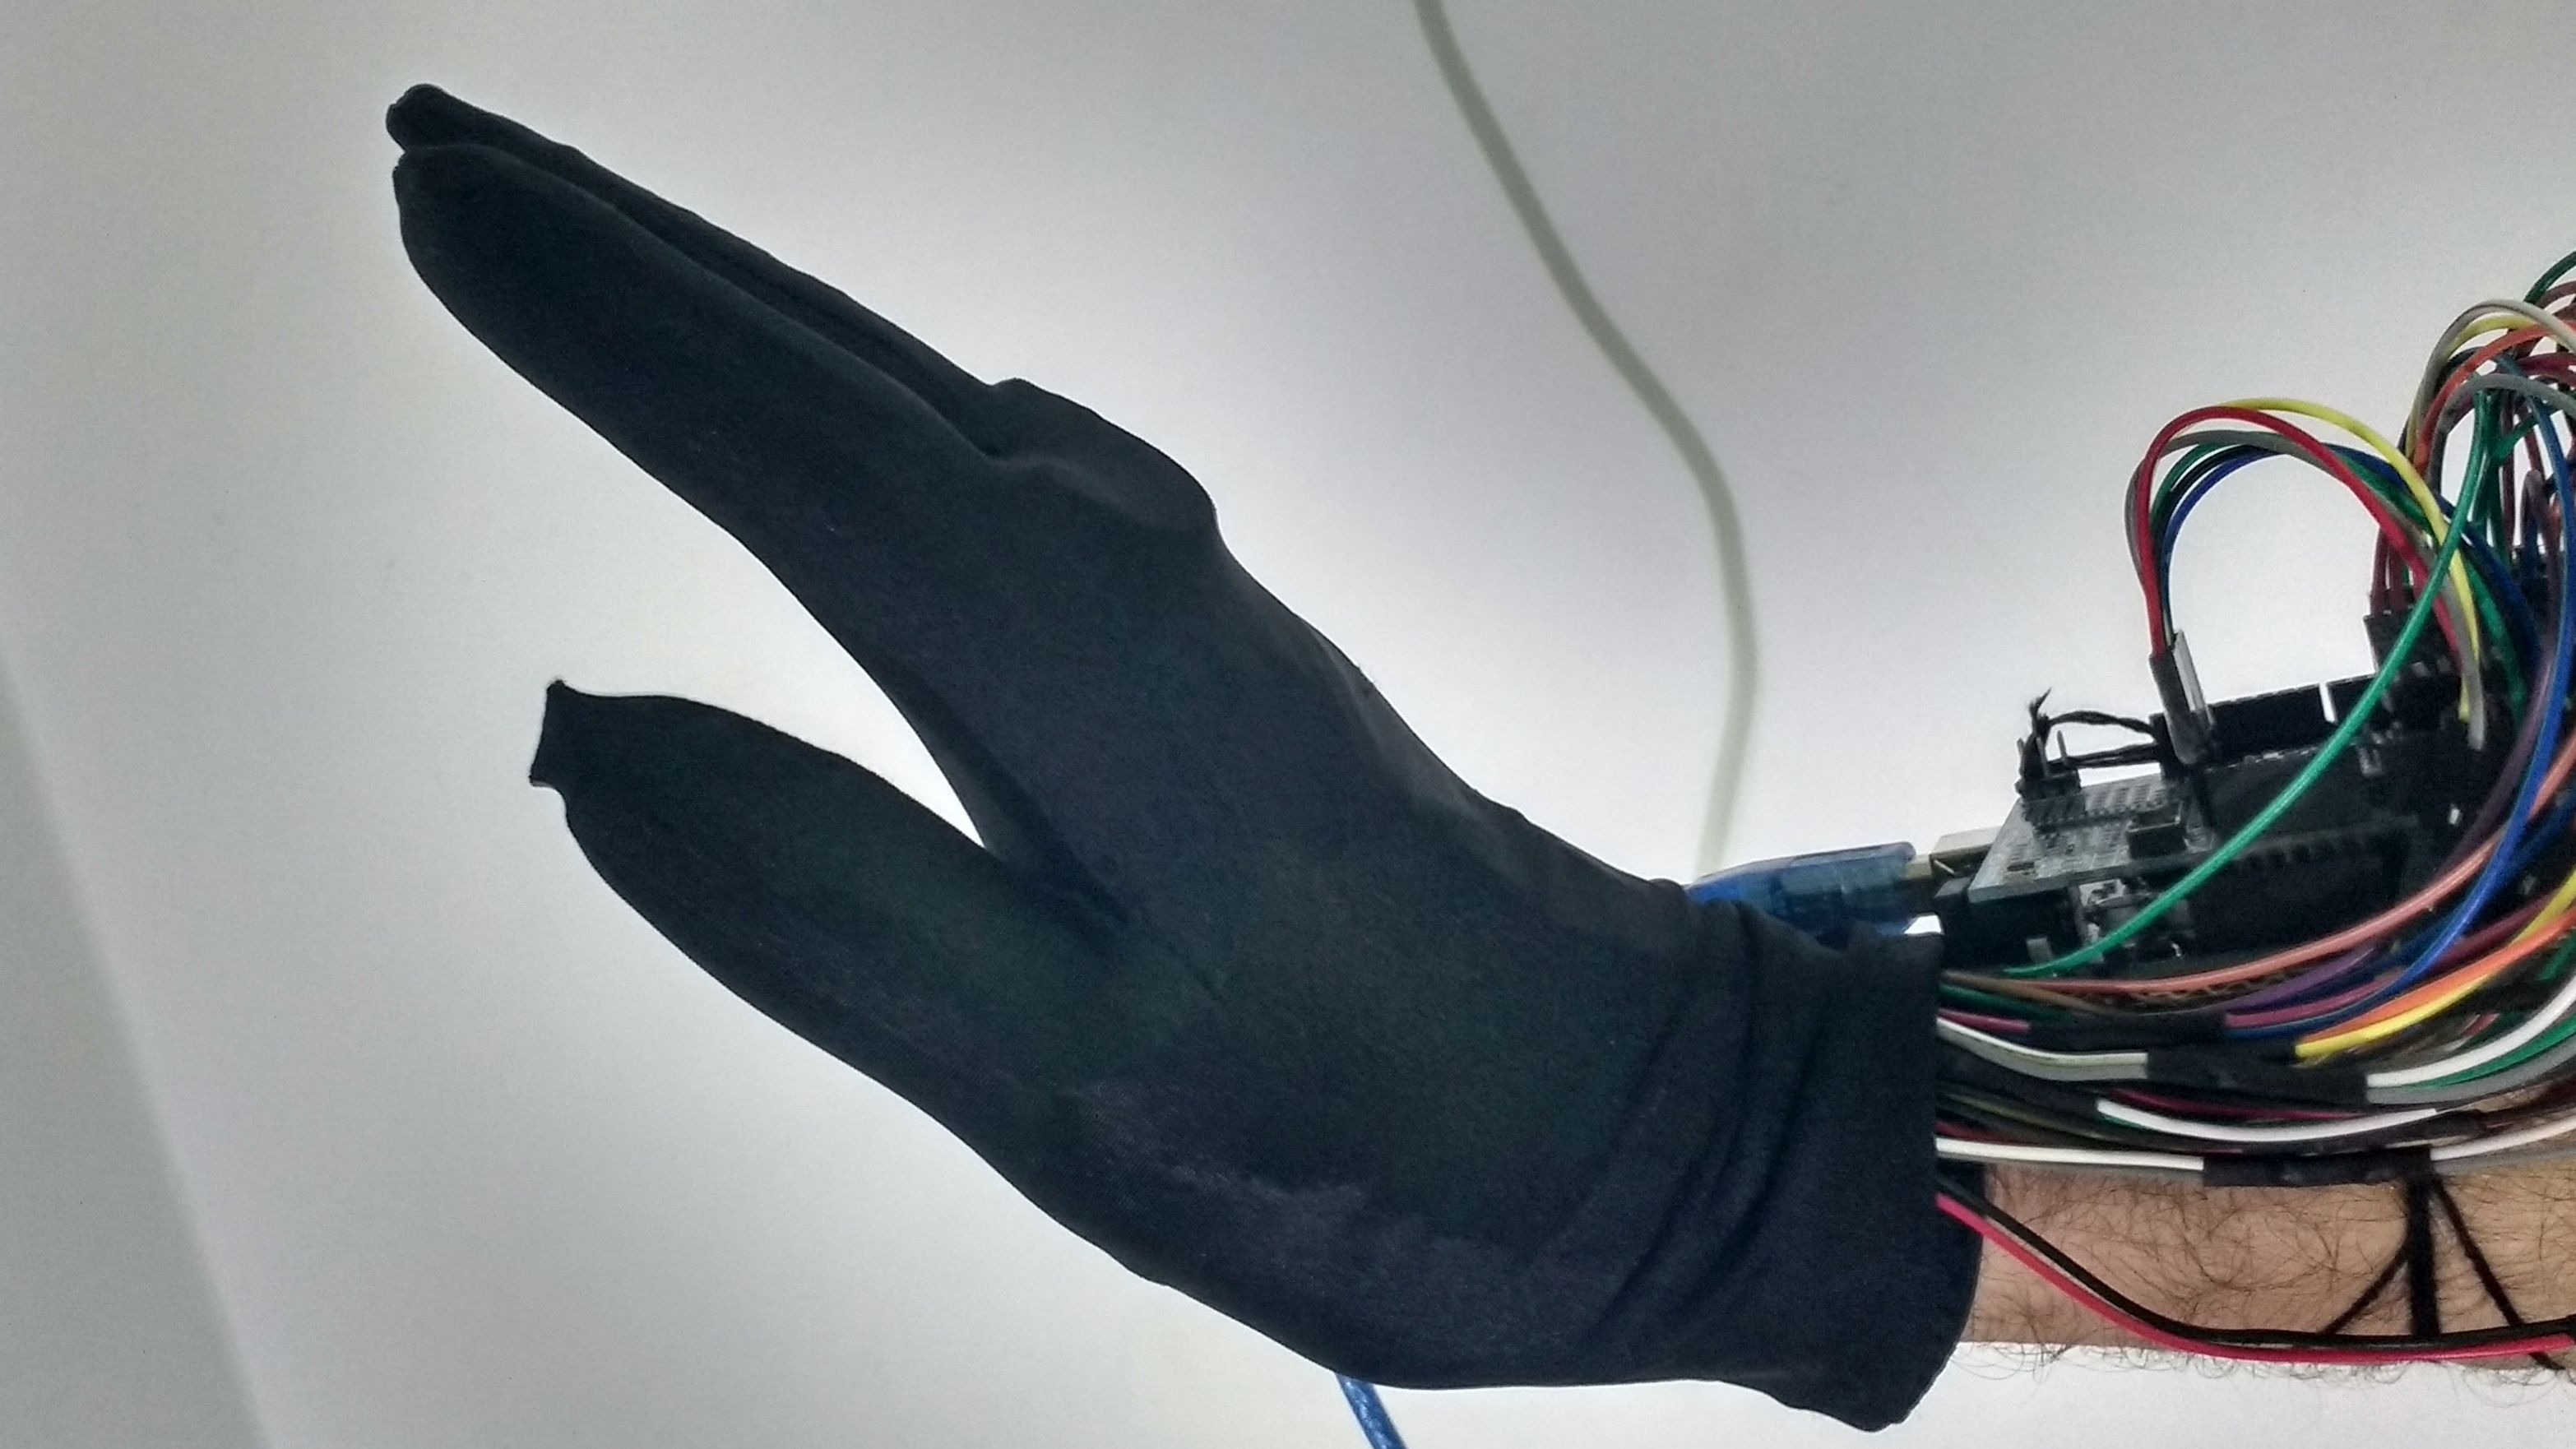
\includegraphics[width=.4\textwidth]{imagem/p6_real}\label{fig:pos_6_real}}
  \quad
  \subfloat[Posição 6 - Modelo]{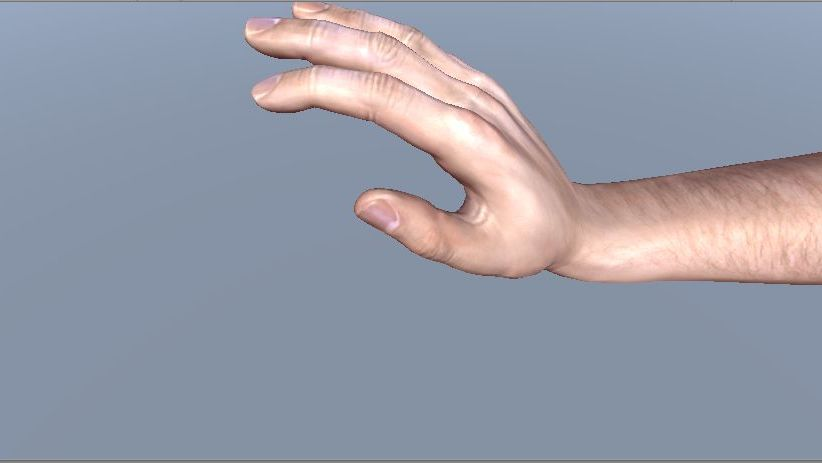
\includegraphics[width=.4\textwidth]{imagem/p6}\label{fig:pos_6_modelo}}\\
  \subfloat[Posição 7 - Real]{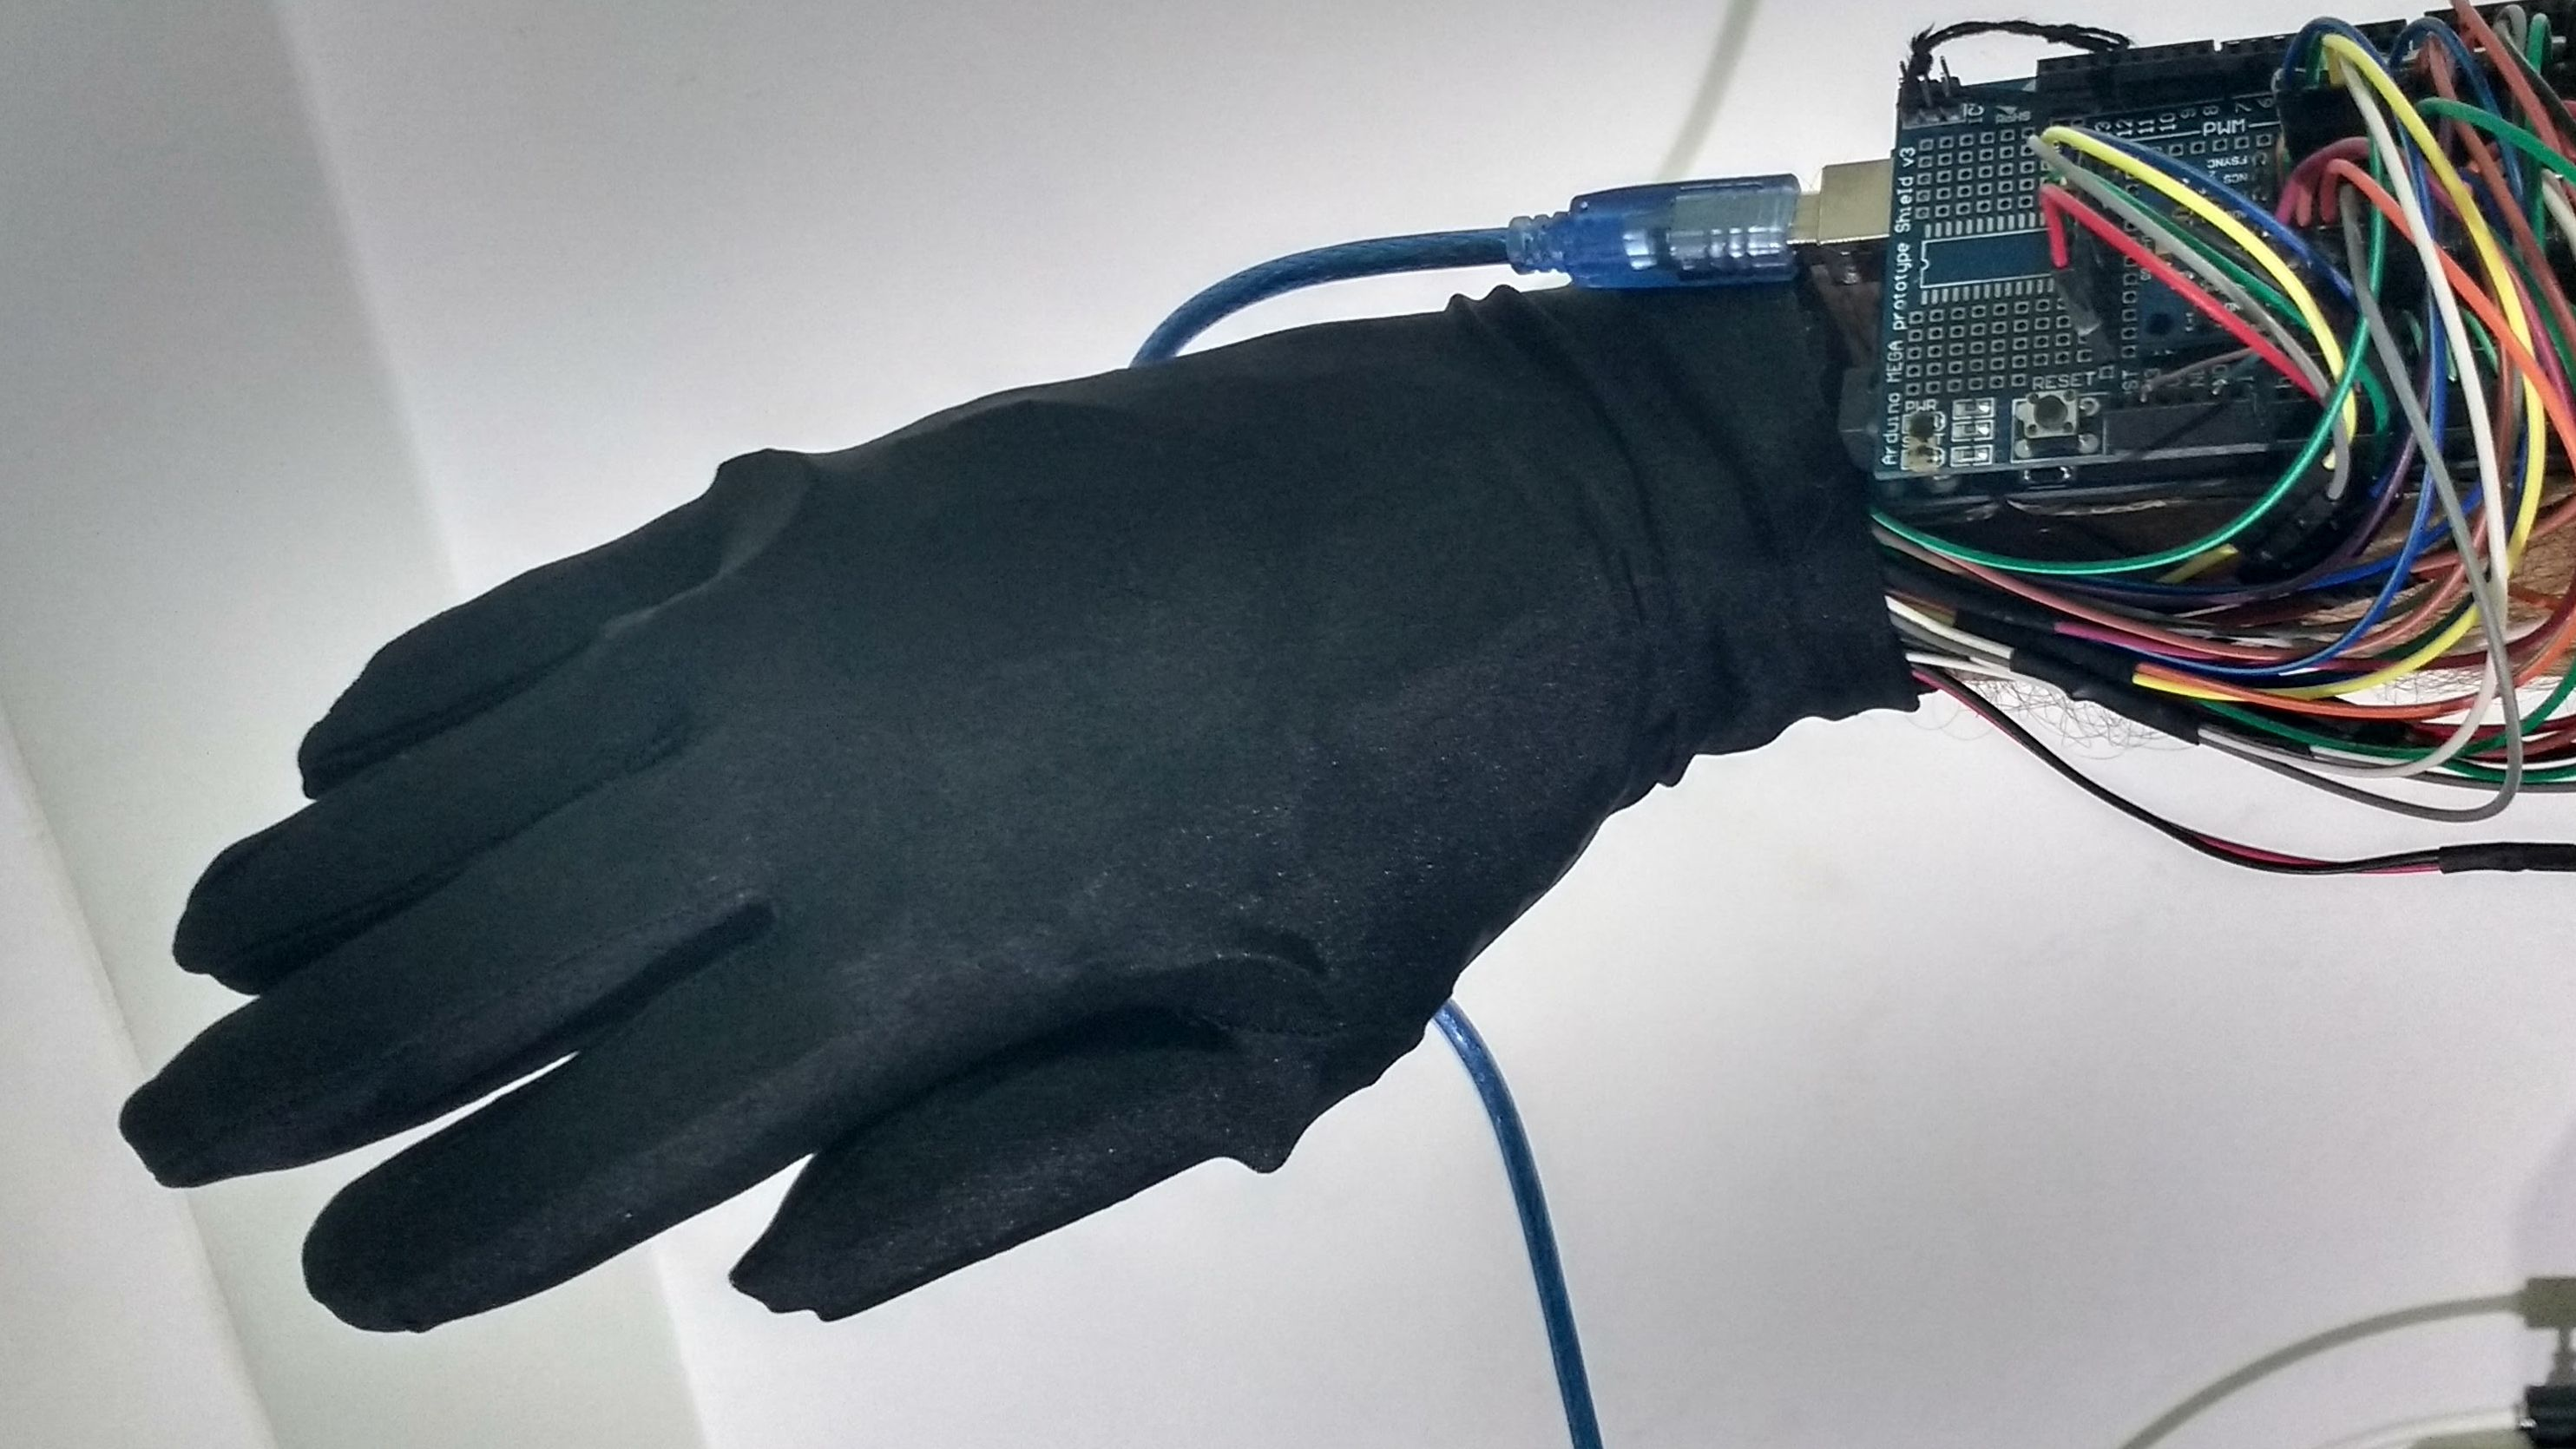
\includegraphics[width=.4\textwidth]{imagem/p7_real}\label{fig:pos_7_real}}
  \quad
  \subfloat[Posição 7 - Modelo]{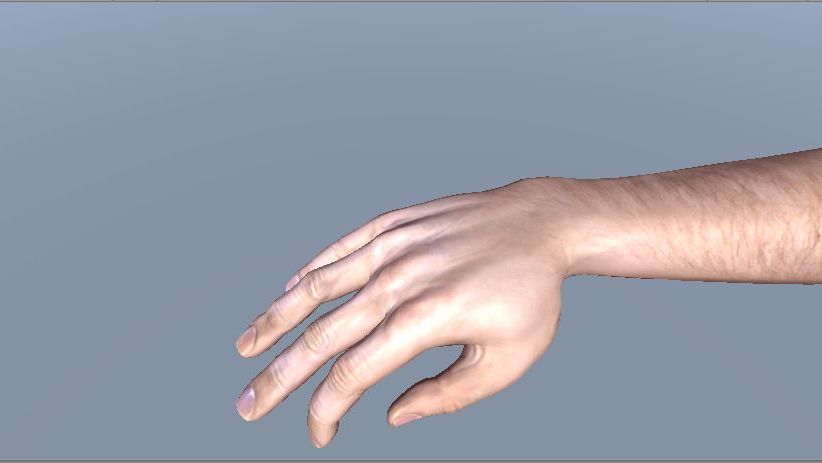
\includegraphics[width=.4\textwidth]{imagem/p7}\label{fig:pos_7_modelo}}\\
  \subfloat[Posição 8 - Real]{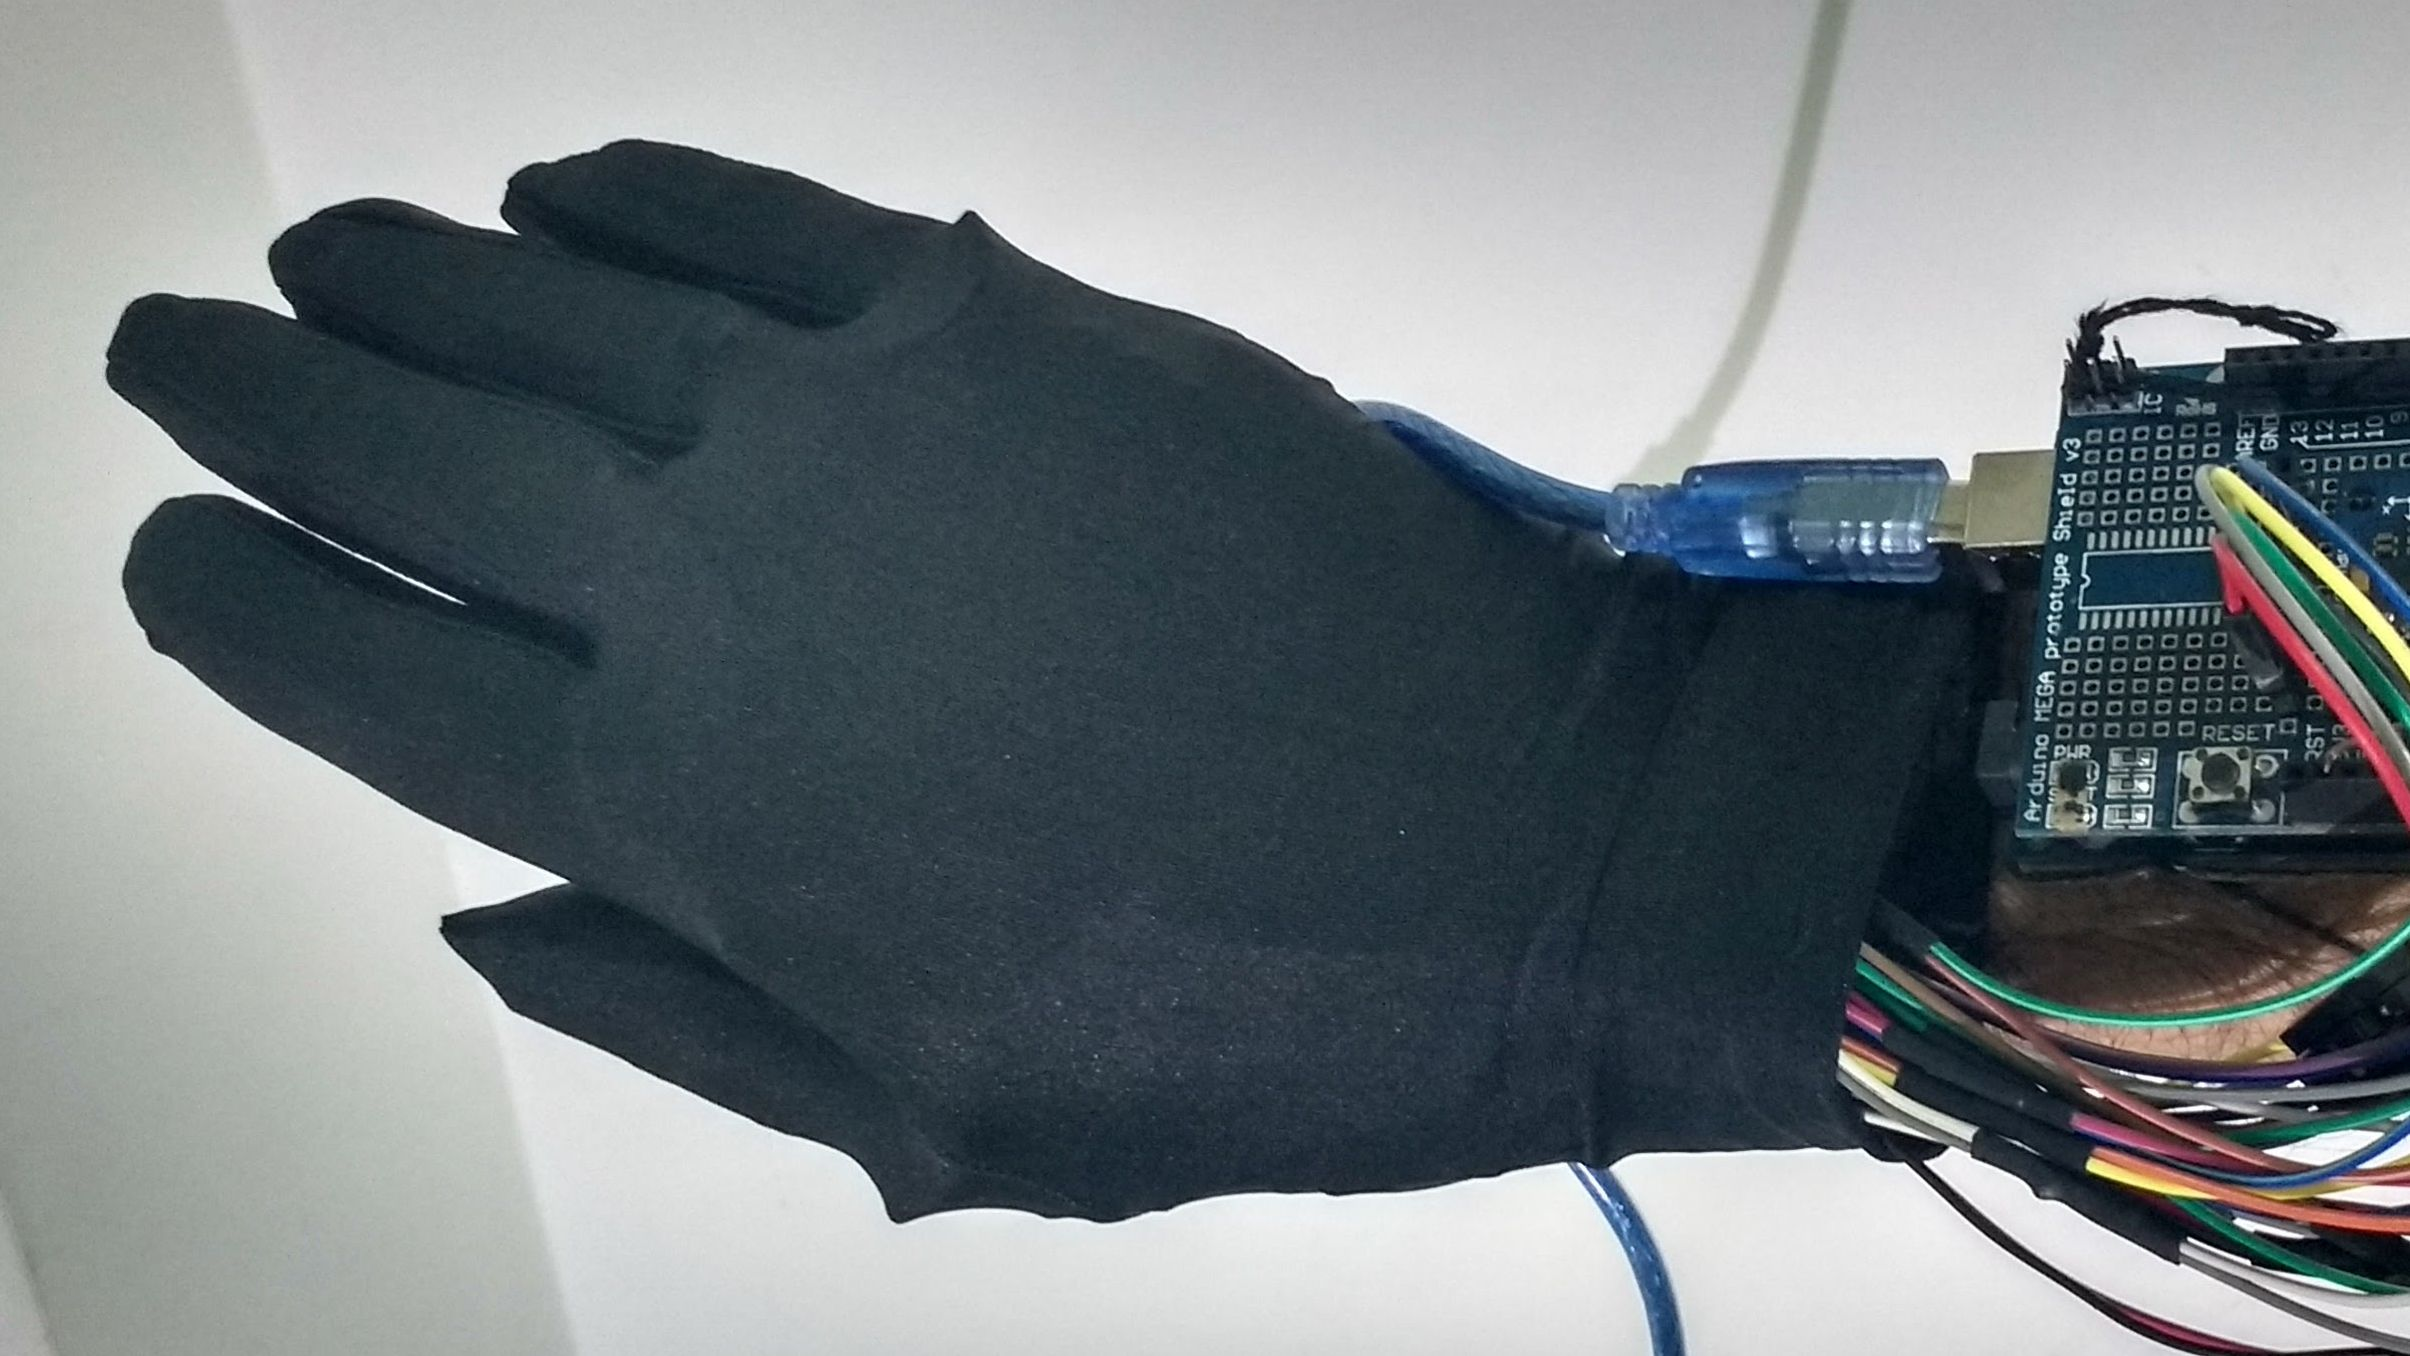
\includegraphics[width=.4\textwidth]{imagem/p8_real}\label{fig:pos_8_real}}
  \quad
  \subfloat[Posição 8 - Modelo]{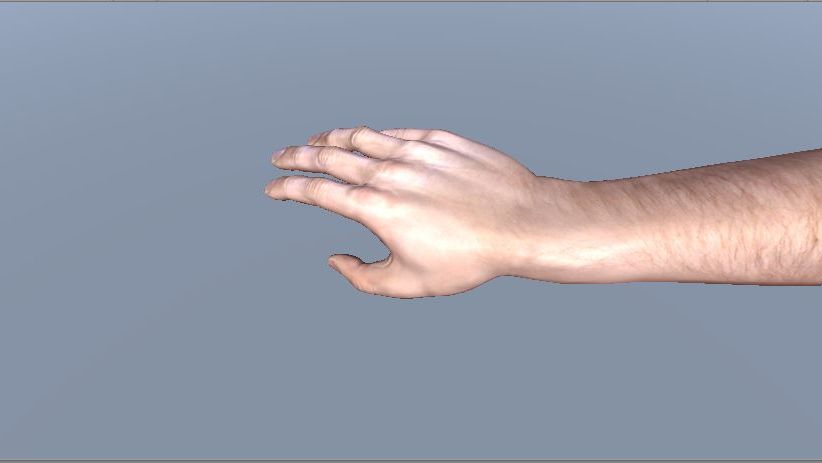
\includegraphics[width=.4\textwidth]{imagem/p8}\label{fig:pos_8_modelo}}\\
  \subfloat[Posição 9 - Real]{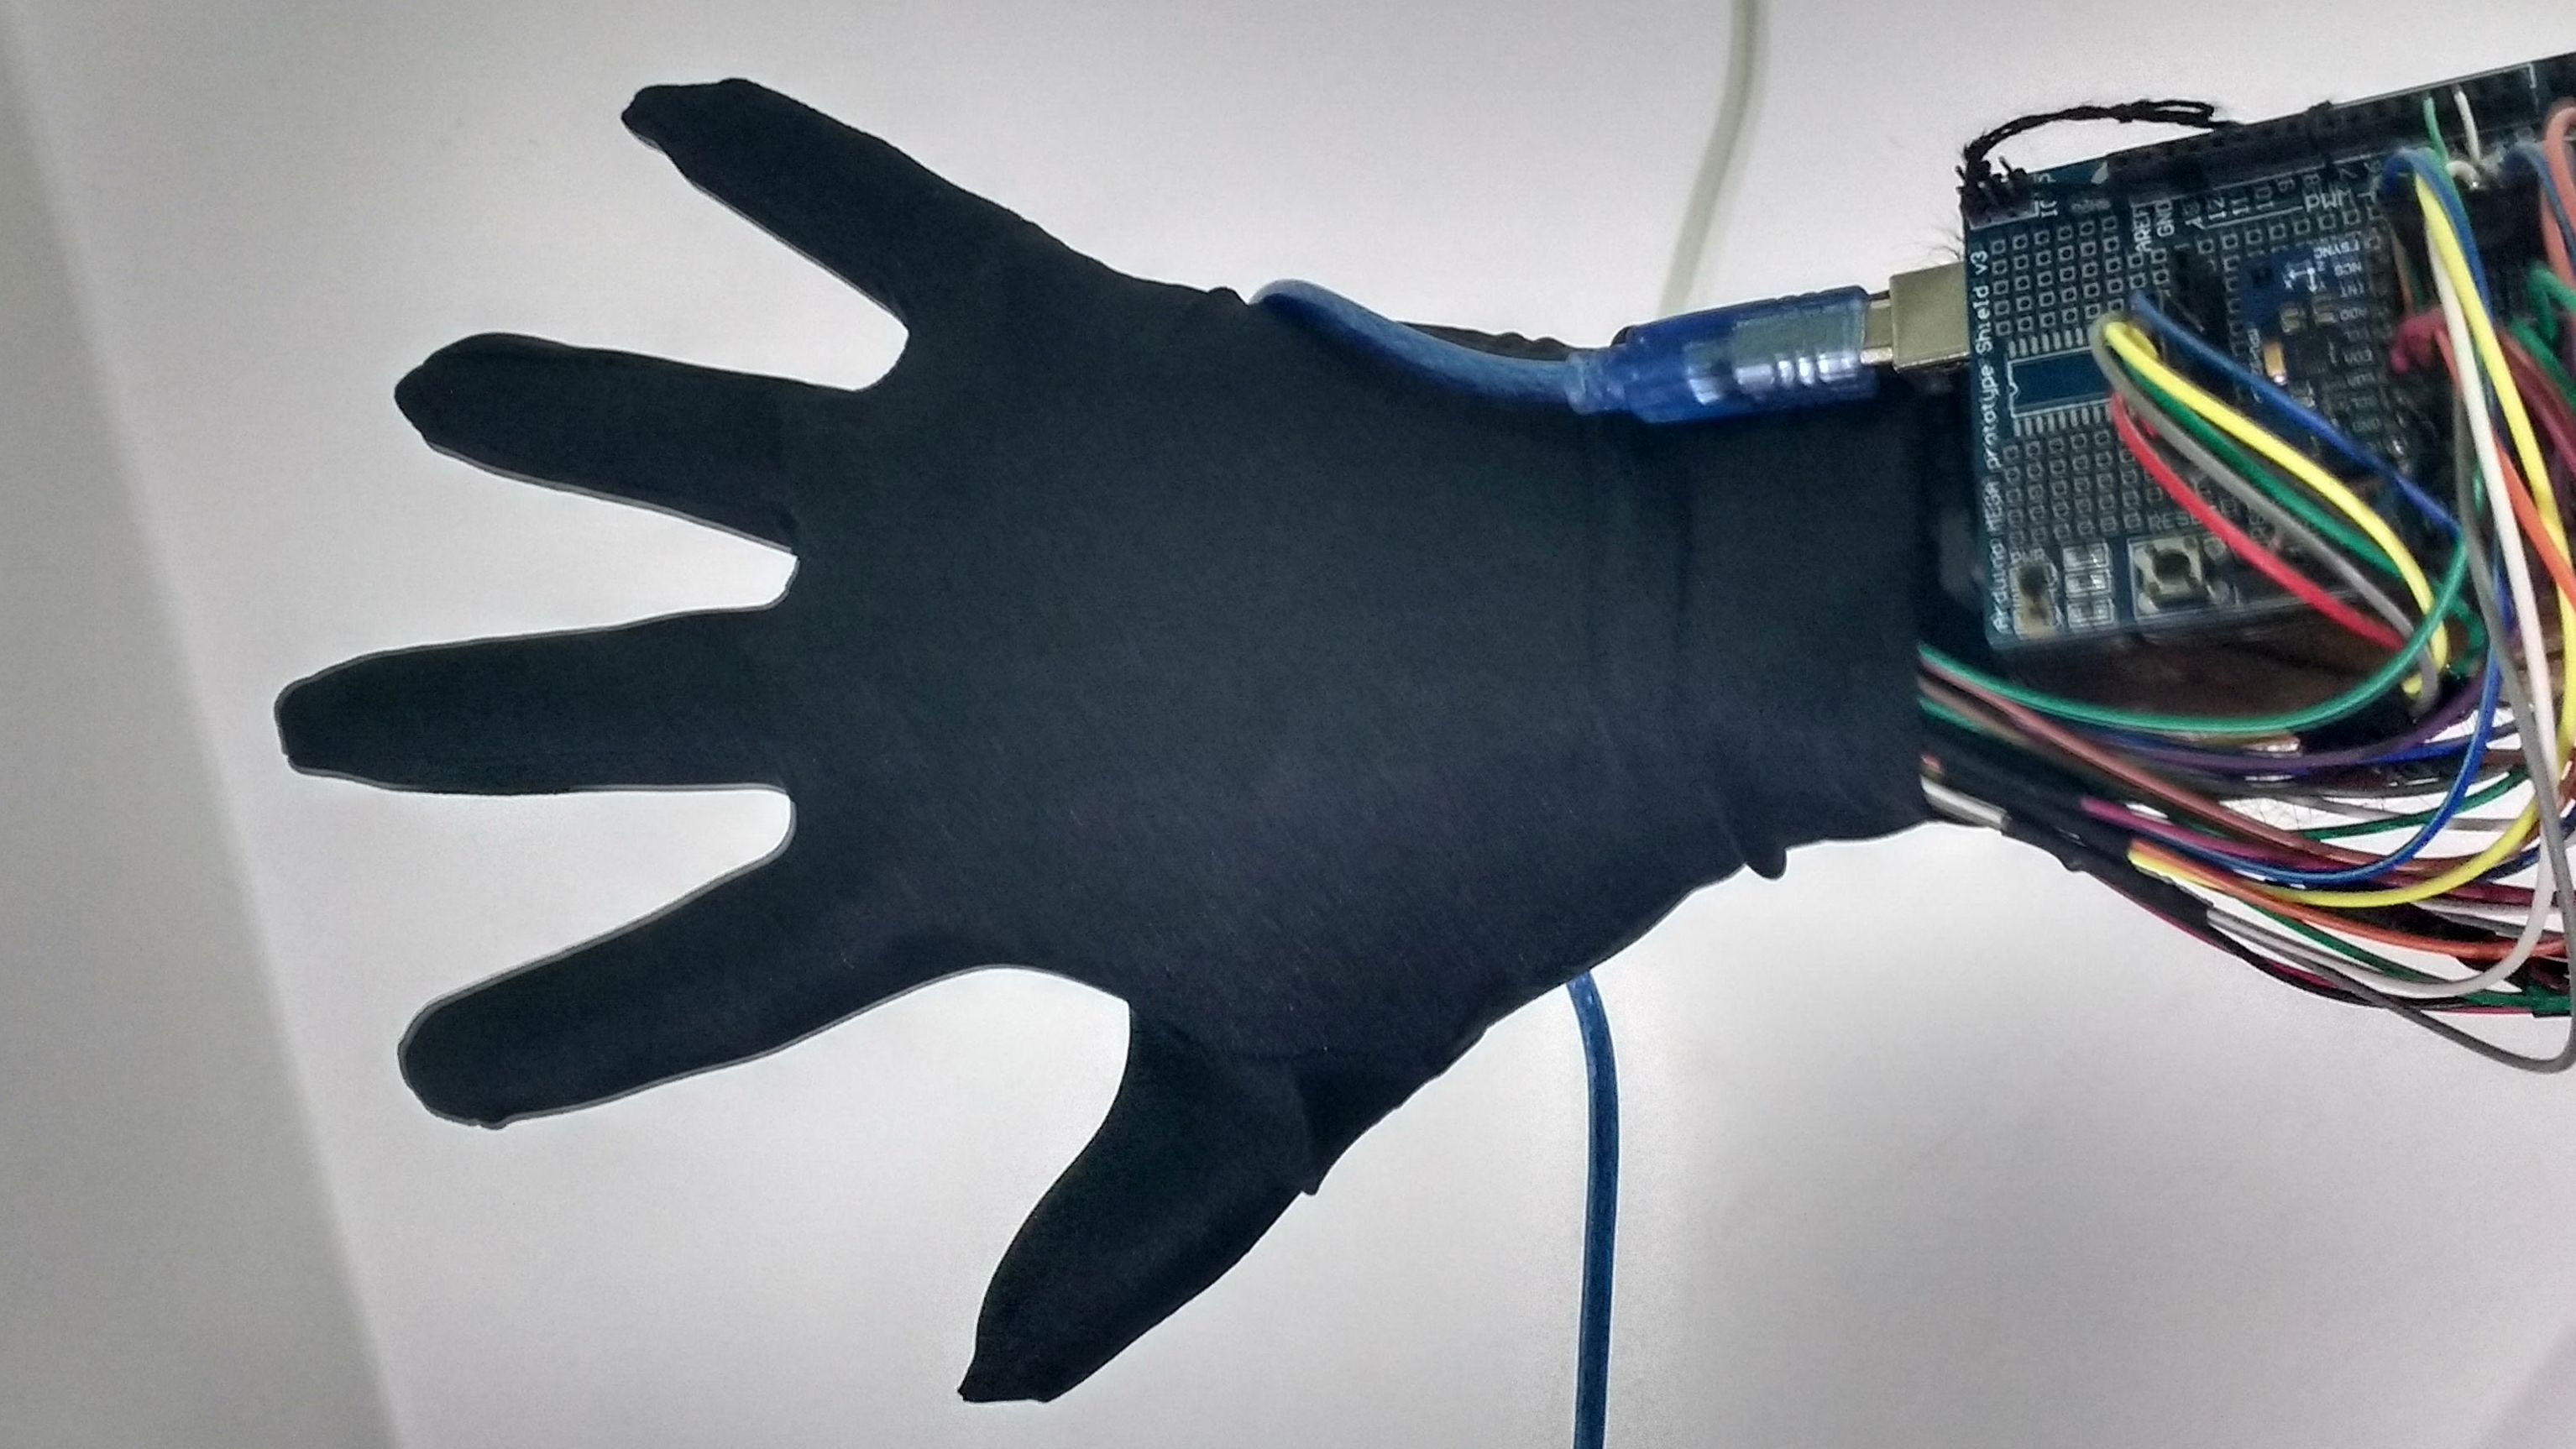
\includegraphics[width=.4\textwidth]{imagem/p9_real}\label{fig:pos_9_real}}
  \quad
  \subfloat[Posição 9 - Modelo]{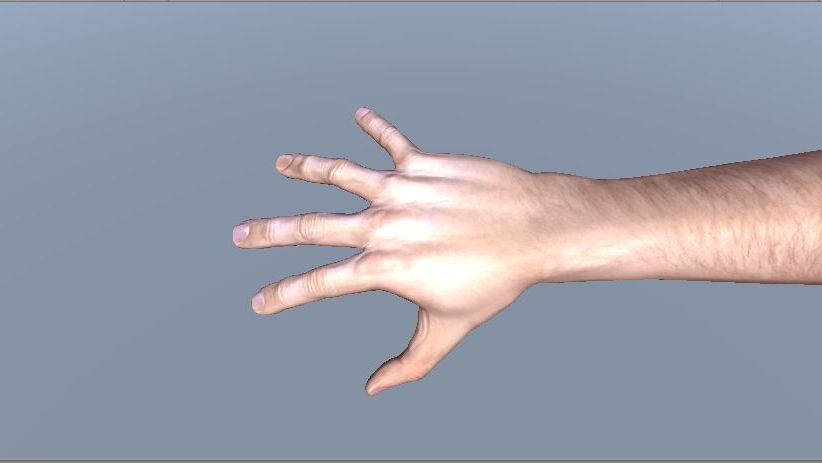
\includegraphics[width=.4\textwidth]{imagem/p9}\label{fig:pos_9_modelo}}\\
  \captionsetup{justification=centering}
  \captionfont{\small{\textbf{\\Fonte: Elaborado pelo Autor}}}
  \label{fig:pos_res2}
\end{figure}

\section{Problemas encontrados}
\label{sec:prob}

Após a montagem da luva, o sensor da articulação \ac{IFP} do anelar apresentou ruídos excessivos, mesmo após a aplicação do filtro. As possíveis causas são o mau funcionamento do sensor, ou curto-circuitos causados pela interação com os outros sensores próximos a ele.

Foi observado que valores usados na conversão para o ângulo de dobra dos sensores de flexão podem variar quando o circuito é alterado, ou até mesmo após a recolocação da luva. Essa alteração ocorre devido às variações na posição do tecido da luva, fazendo com que os sensores não fiquem na mesma posição.

Os sensores usados na detecção dos movimentos de adução e abdução eram influenciados pelos movimentos de flexão dos dedos, devido à sua posição na luva (Figura \ref{fig:pos_indic}). Ao estender apenas o dedo indicador, o sensor entre os dedos indicador e médio era deformado, gerando leituras que causavam a abdução desse dedo no modelo \ac{3D}. Para solucionar esse problema deveriam ser criadas regras para ignorar leituras dos sensores de abdução quando apenas um dos dedos se movimentasse.

O tecido da luva e o posicionamento do \textit{Arduino} limitaram certos movimentos como o movimento de abdução do polegar e o de extensão do pulso, que foi interferido pelo cabo \ac{USB}.

\begin{figure}[H]
  \setlength{\abovecaptionskip}{0pt}
  \setlength{\belowcaptionskip}{0pt}
  \caption[Movimentação errada ao estender apenas o dedo indicador]{Movimentação errada ao estender apenas o dedo indicador}
  \centering
  \subfloat[Extensão - Real]{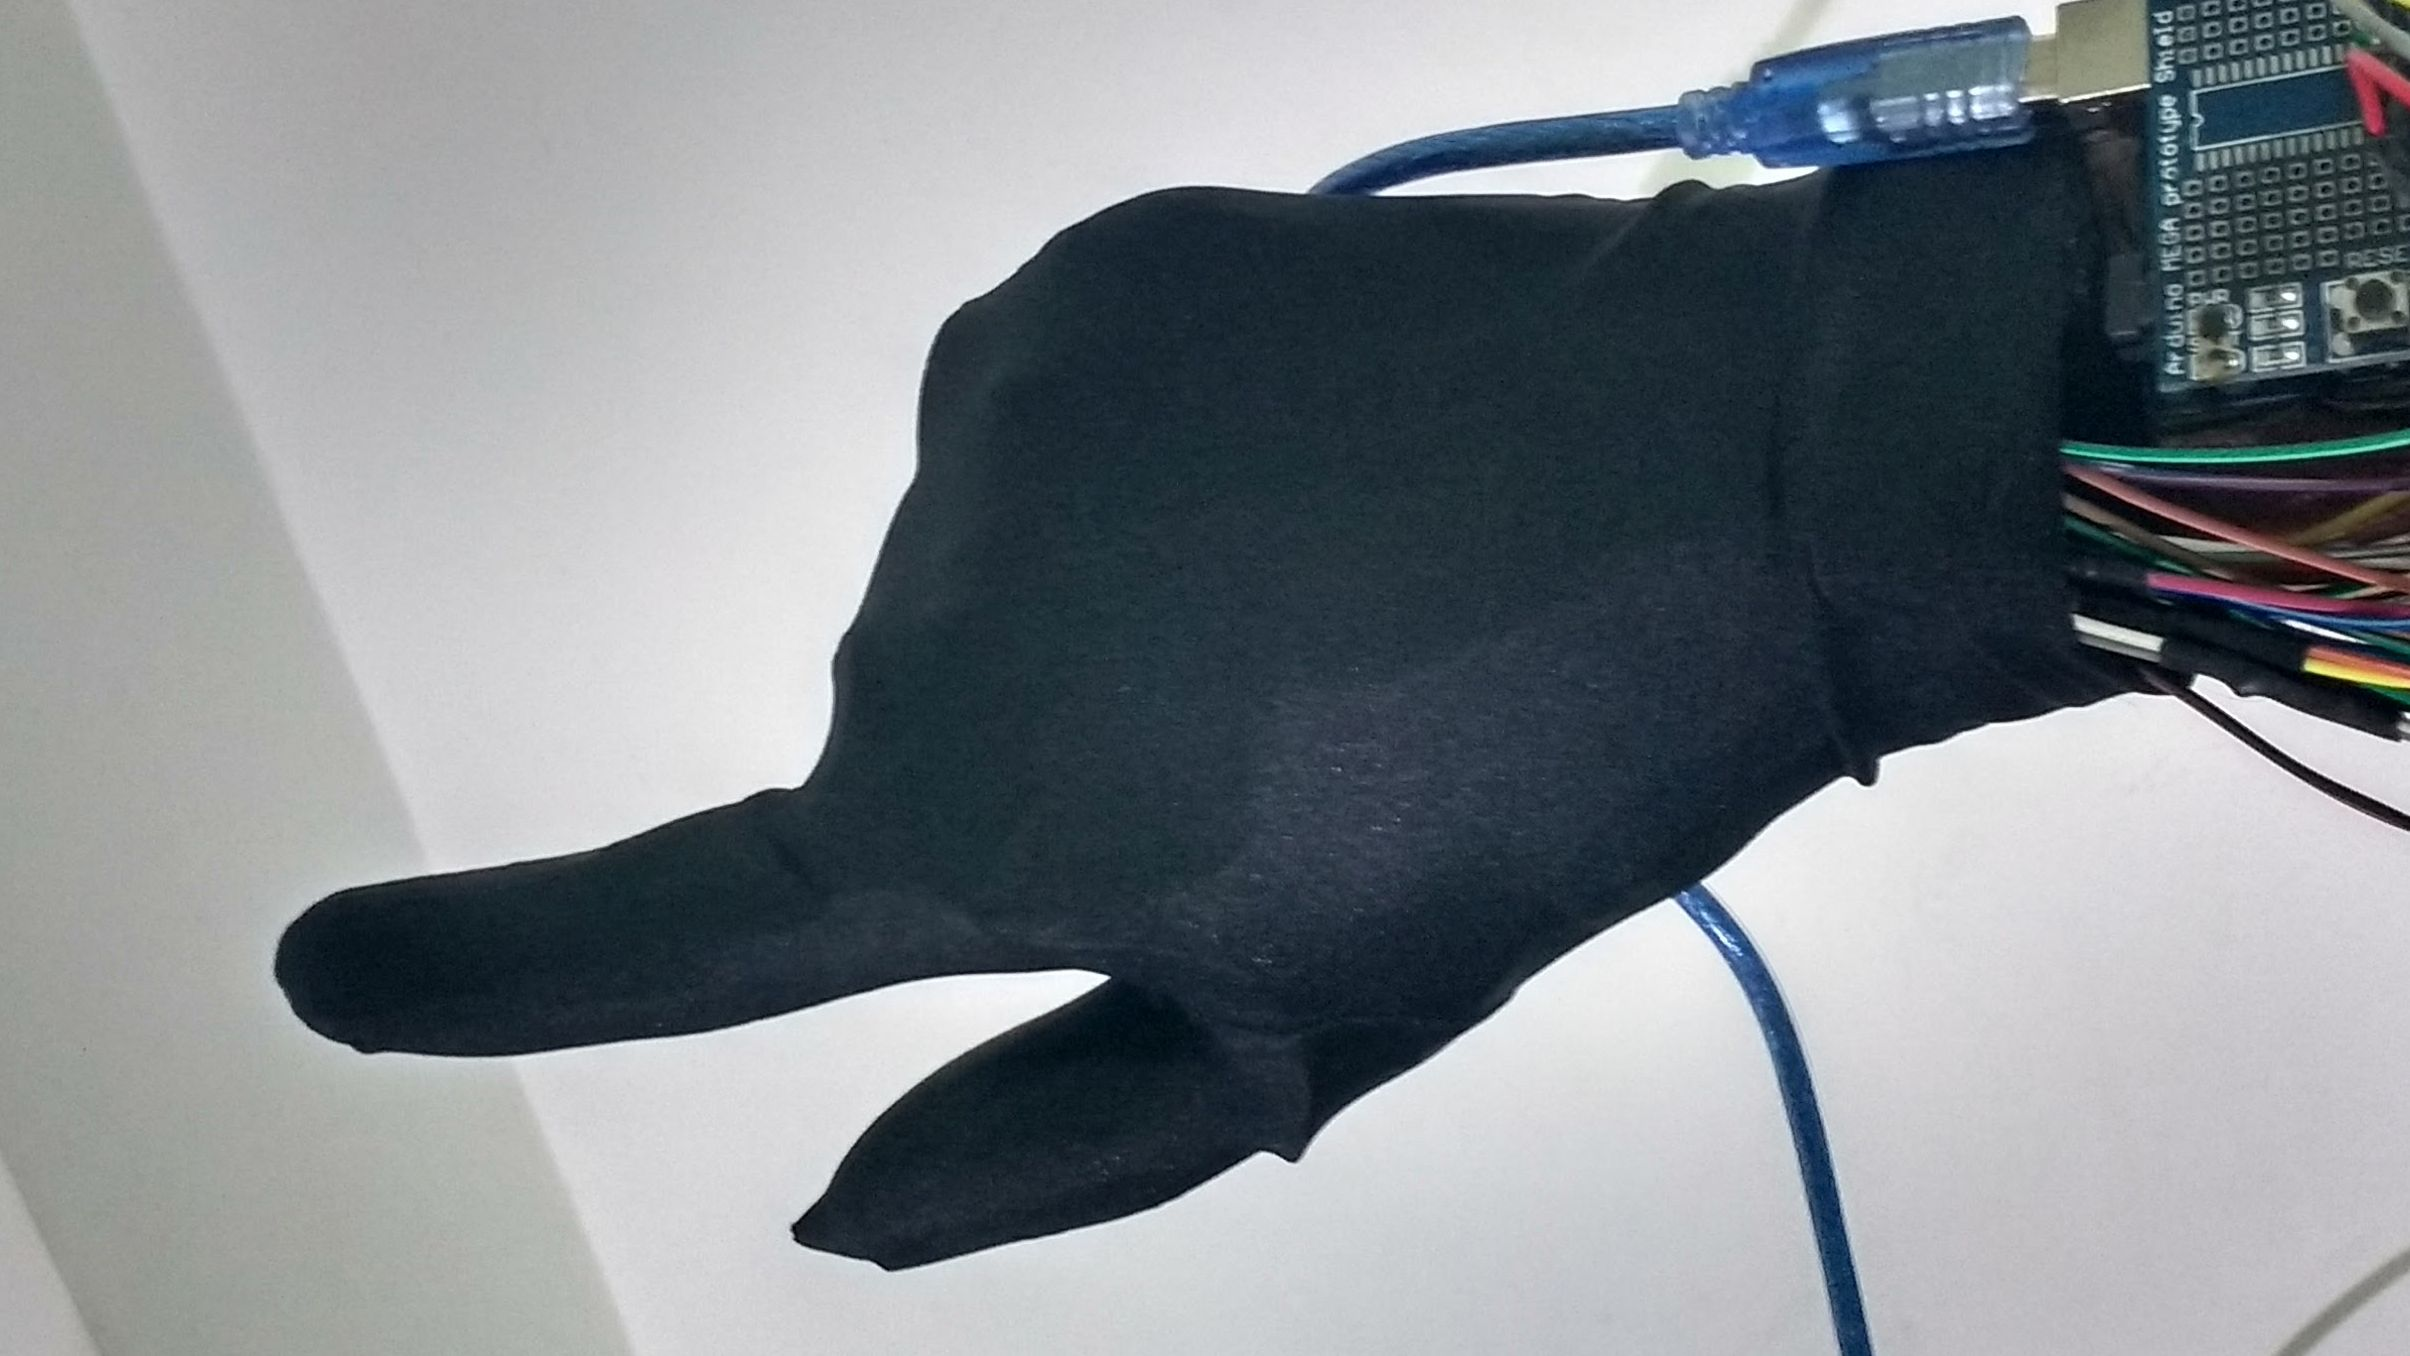
\includegraphics[width=.4\textwidth]{imagem/indicadorabducao_real}\label{fig:indicadorabducao_real}}
  \quad
  \subfloat[Extensão e abdução - Modelo]{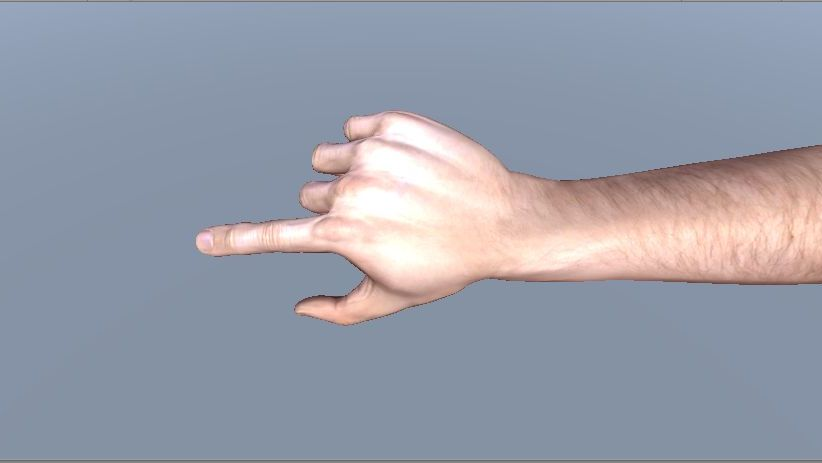
\includegraphics[width=.4\textwidth]{imagem/indicadorabducao}\label{fig:indicadorabducao_modelo}}\\
  \captionsetup{justification=centering}
  \captionfont{\small{\textbf{\\Fonte: Elaborado pelo Autor}}}
  \label{fig:pos_indic}
\end{figure}


% Texto do capítulo